\documentclass{article}
\usepackage{iclr2027_conference,times}
%%%%% NEW MATH DEFINITIONS %%%%%

\usepackage{amsmath,amsfonts,bm}

% Mark sections of captions for referring to divisions of figures
\newcommand{\figleft}{{\em (Left)}}
\newcommand{\figcenter}{{\em (Center)}}
\newcommand{\figright}{{\em (Right)}}
\newcommand{\figtop}{{\em (Top)}}
\newcommand{\figbottom}{{\em (Bottom)}}
\newcommand{\captiona}{{\em (a)}}
\newcommand{\captionb}{{\em (b)}}
\newcommand{\captionc}{{\em (c)}}
\newcommand{\captiond}{{\em (d)}}

% Highlight a newly defined term
\newcommand{\newterm}[1]{{\bf #1}}


% Figure reference, lower-case.
\def\figref#1{figure~\ref{#1}}
% Figure reference, capital. For start of sentence
\def\Figref#1{Figure~\ref{#1}}
\def\twofigref#1#2{figures \ref{#1} and \ref{#2}}
\def\quadfigref#1#2#3#4{figures \ref{#1}, \ref{#2}, \ref{#3} and \ref{#4}}
% Section reference, lower-case.
\def\secref#1{section~\ref{#1}}
% Section reference, capital.
\def\Secref#1{Section~\ref{#1}}
% Reference to two sections.
\def\twosecrefs#1#2{sections \ref{#1} and \ref{#2}}
% Reference to three sections.
\def\secrefs#1#2#3{sections \ref{#1}, \ref{#2} and \ref{#3}}
% Reference to an equation, lower-case.
\def\eqref#1{equation~\ref{#1}}
% Reference to an equation, upper case
\def\Eqref#1{Equation~\ref{#1}}
% A raw reference to an equation---avoid using if possible
\def\plaineqref#1{\ref{#1}}
% Reference to a chapter, lower-case.
\def\chapref#1{chapter~\ref{#1}}
% Reference to an equation, upper case.
\def\Chapref#1{Chapter~\ref{#1}}
% Reference to a range of chapters
\def\rangechapref#1#2{chapters\ref{#1}--\ref{#2}}
% Reference to an algorithm, lower-case.
\def\algref#1{algorithm~\ref{#1}}
% Reference to an algorithm, upper case.
\def\Algref#1{Algorithm~\ref{#1}}
\def\twoalgref#1#2{algorithms \ref{#1} and \ref{#2}}
\def\Twoalgref#1#2{Algorithms \ref{#1} and \ref{#2}}
% Reference to a part, lower case
\def\partref#1{part~\ref{#1}}
% Reference to a part, upper case
\def\Partref#1{Part~\ref{#1}}
\def\twopartref#1#2{parts \ref{#1} and \ref{#2}}

\def\ceil#1{\lceil #1 \rceil}
\def\floor#1{\lfloor #1 \rfloor}
\def\1{\bm{1}}
\newcommand{\train}{\mathcal{D}}
\newcommand{\valid}{\mathcal{D_{\mathrm{valid}}}}
\newcommand{\test}{\mathcal{D_{\mathrm{test}}}}

\def\eps{{\epsilon}}


% Random variables
\def\reta{{\textnormal{$\eta$}}}
\def\ra{{\textnormal{a}}}
\def\rb{{\textnormal{b}}}
\def\rc{{\textnormal{c}}}
\def\rd{{\textnormal{d}}}
\def\re{{\textnormal{e}}}
\def\rf{{\textnormal{f}}}
\def\rg{{\textnormal{g}}}
\def\rh{{\textnormal{h}}}
\def\ri{{\textnormal{i}}}
\def\rj{{\textnormal{j}}}
\def\rk{{\textnormal{k}}}
\def\rl{{\textnormal{l}}}
% rm is already a command, just don't name any random variables m
\def\rn{{\textnormal{n}}}
\def\ro{{\textnormal{o}}}
\def\rp{{\textnormal{p}}}
\def\rq{{\textnormal{q}}}
\def\rr{{\textnormal{r}}}
\def\rs{{\textnormal{s}}}
\def\rt{{\textnormal{t}}}
\def\ru{{\textnormal{u}}}
\def\rv{{\textnormal{v}}}
\def\rw{{\textnormal{w}}}
\def\rx{{\textnormal{x}}}
\def\ry{{\textnormal{y}}}
\def\rz{{\textnormal{z}}}

% Random vectors
\def\rvepsilon{{\mathbf{\epsilon}}}
\def\rvtheta{{\mathbf{\theta}}}
\def\rva{{\mathbf{a}}}
\def\rvb{{\mathbf{b}}}
\def\rvc{{\mathbf{c}}}
\def\rvd{{\mathbf{d}}}
\def\rve{{\mathbf{e}}}
\def\rvf{{\mathbf{f}}}
\def\rvg{{\mathbf{g}}}
\def\rvh{{\mathbf{h}}}
\def\rvu{{\mathbf{i}}}
\def\rvj{{\mathbf{j}}}
\def\rvk{{\mathbf{k}}}
\def\rvl{{\mathbf{l}}}
\def\rvm{{\mathbf{m}}}
\def\rvn{{\mathbf{n}}}
\def\rvo{{\mathbf{o}}}
\def\rvp{{\mathbf{p}}}
\def\rvq{{\mathbf{q}}}
\def\rvr{{\mathbf{r}}}
\def\rvs{{\mathbf{s}}}
\def\rvt{{\mathbf{t}}}
\def\rvu{{\mathbf{u}}}
\def\rvv{{\mathbf{v}}}
\def\rvw{{\mathbf{w}}}
\def\rvx{{\mathbf{x}}}
\def\rvy{{\mathbf{y}}}
\def\rvz{{\mathbf{z}}}

% Elements of random vectors
\def\erva{{\textnormal{a}}}
\def\ervb{{\textnormal{b}}}
\def\ervc{{\textnormal{c}}}
\def\ervd{{\textnormal{d}}}
\def\erve{{\textnormal{e}}}
\def\ervf{{\textnormal{f}}}
\def\ervg{{\textnormal{g}}}
\def\ervh{{\textnormal{h}}}
\def\ervi{{\textnormal{i}}}
\def\ervj{{\textnormal{j}}}
\def\ervk{{\textnormal{k}}}
\def\ervl{{\textnormal{l}}}
\def\ervm{{\textnormal{m}}}
\def\ervn{{\textnormal{n}}}
\def\ervo{{\textnormal{o}}}
\def\ervp{{\textnormal{p}}}
\def\ervq{{\textnormal{q}}}
\def\ervr{{\textnormal{r}}}
\def\ervs{{\textnormal{s}}}
\def\ervt{{\textnormal{t}}}
\def\ervu{{\textnormal{u}}}
\def\ervv{{\textnormal{v}}}
\def\ervw{{\textnormal{w}}}
\def\ervx{{\textnormal{x}}}
\def\ervy{{\textnormal{y}}}
\def\ervz{{\textnormal{z}}}

% Random matrices
\def\rmA{{\mathbf{A}}}
\def\rmB{{\mathbf{B}}}
\def\rmC{{\mathbf{C}}}
\def\rmD{{\mathbf{D}}}
\def\rmE{{\mathbf{E}}}
\def\rmF{{\mathbf{F}}}
\def\rmG{{\mathbf{G}}}
\def\rmH{{\mathbf{H}}}
\def\rmI{{\mathbf{I}}}
\def\rmJ{{\mathbf{J}}}
\def\rmK{{\mathbf{K}}}
\def\rmL{{\mathbf{L}}}
\def\rmM{{\mathbf{M}}}
\def\rmN{{\mathbf{N}}}
\def\rmO{{\mathbf{O}}}
\def\rmP{{\mathbf{P}}}
\def\rmQ{{\mathbf{Q}}}
\def\rmR{{\mathbf{R}}}
\def\rmS{{\mathbf{S}}}
\def\rmT{{\mathbf{T}}}
\def\rmU{{\mathbf{U}}}
\def\rmV{{\mathbf{V}}}
\def\rmW{{\mathbf{W}}}
\def\rmX{{\mathbf{X}}}
\def\rmY{{\mathbf{Y}}}
\def\rmZ{{\mathbf{Z}}}

% Elements of random matrices
\def\ermA{{\textnormal{A}}}
\def\ermB{{\textnormal{B}}}
\def\ermC{{\textnormal{C}}}
\def\ermD{{\textnormal{D}}}
\def\ermE{{\textnormal{E}}}
\def\ermF{{\textnormal{F}}}
\def\ermG{{\textnormal{G}}}
\def\ermH{{\textnormal{H}}}
\def\ermI{{\textnormal{I}}}
\def\ermJ{{\textnormal{J}}}
\def\ermK{{\textnormal{K}}}
\def\ermL{{\textnormal{L}}}
\def\ermM{{\textnormal{M}}}
\def\ermN{{\textnormal{N}}}
\def\ermO{{\textnormal{O}}}
\def\ermP{{\textnormal{P}}}
\def\ermQ{{\textnormal{Q}}}
\def\ermR{{\textnormal{R}}}
\def\ermS{{\textnormal{S}}}
\def\ermT{{\textnormal{T}}}
\def\ermU{{\textnormal{U}}}
\def\ermV{{\textnormal{V}}}
\def\ermW{{\textnormal{W}}}
\def\ermX{{\textnormal{X}}}
\def\ermY{{\textnormal{Y}}}
\def\ermZ{{\textnormal{Z}}}

% Vectors
\def\vzero{{\bm{0}}}
\def\vone{{\bm{1}}}
\def\vmu{{\bm{\mu}}}
\def\vtheta{{\bm{\theta}}}
\def\va{{\bm{a}}}
\def\vb{{\bm{b}}}
\def\vc{{\bm{c}}}
\def\vd{{\bm{d}}}
\def\ve{{\bm{e}}}
\def\vf{{\bm{f}}}
\def\vg{{\bm{g}}}
\def\vh{{\bm{h}}}
\def\vi{{\bm{i}}}
\def\vj{{\bm{j}}}
\def\vk{{\bm{k}}}
\def\vl{{\bm{l}}}
\def\vm{{\bm{m}}}
\def\vn{{\bm{n}}}
\def\vo{{\bm{o}}}
\def\vp{{\bm{p}}}
\def\vq{{\bm{q}}}
\def\vr{{\bm{r}}}
\def\vs{{\bm{s}}}
\def\vt{{\bm{t}}}
\def\vu{{\bm{u}}}
\def\vv{{\bm{v}}}
\def\vw{{\bm{w}}}
\def\vx{{\bm{x}}}
\def\vy{{\bm{y}}}
\def\vz{{\bm{z}}}

% Elements of vectors
\def\evalpha{{\alpha}}
\def\evbeta{{\beta}}
\def\evepsilon{{\epsilon}}
\def\evlambda{{\lambda}}
\def\evomega{{\omega}}
\def\evmu{{\mu}}
\def\evpsi{{\psi}}
\def\evsigma{{\sigma}}
\def\evtheta{{\theta}}
\def\eva{{a}}
\def\evb{{b}}
\def\evc{{c}}
\def\evd{{d}}
\def\eve{{e}}
\def\evf{{f}}
\def\evg{{g}}
\def\evh{{h}}
\def\evi{{i}}
\def\evj{{j}}
\def\evk{{k}}
\def\evl{{l}}
\def\evm{{m}}
\def\evn{{n}}
\def\evo{{o}}
\def\evp{{p}}
\def\evq{{q}}
\def\evr{{r}}
\def\evs{{s}}
\def\evt{{t}}
\def\evu{{u}}
\def\evv{{v}}
\def\evw{{w}}
\def\evx{{x}}
\def\evy{{y}}
\def\evz{{z}}

% Matrix
\def\mA{{\bm{A}}}
\def\mB{{\bm{B}}}
\def\mC{{\bm{C}}}
\def\mD{{\bm{D}}}
\def\mE{{\bm{E}}}
\def\mF{{\bm{F}}}
\def\mG{{\bm{G}}}
\def\mH{{\bm{H}}}
\def\mI{{\bm{I}}}
\def\mJ{{\bm{J}}}
\def\mK{{\bm{K}}}
\def\mL{{\bm{L}}}
\def\mM{{\bm{M}}}
\def\mN{{\bm{N}}}
\def\mO{{\bm{O}}}
\def\mP{{\bm{P}}}
\def\mQ{{\bm{Q}}}
\def\mR{{\bm{R}}}
\def\mS{{\bm{S}}}
\def\mT{{\bm{T}}}
\def\mU{{\bm{U}}}
\def\mV{{\bm{V}}}
\def\mW{{\bm{W}}}
\def\mX{{\bm{X}}}
\def\mY{{\bm{Y}}}
\def\mZ{{\bm{Z}}}
\def\mBeta{{\bm{\beta}}}
\def\mPhi{{\bm{\Phi}}}
\def\mLambda{{\bm{\Lambda}}}
\def\mSigma{{\bm{\Sigma}}}

% Tensor
\DeclareMathAlphabet{\mathsfit}{\encodingdefault}{\sfdefault}{m}{sl}
\SetMathAlphabet{\mathsfit}{bold}{\encodingdefault}{\sfdefault}{bx}{n}
\newcommand{\tens}[1]{\bm{\mathsfit{#1}}}
\def\tA{{\tens{A}}}
\def\tB{{\tens{B}}}
\def\tC{{\tens{C}}}
\def\tD{{\tens{D}}}
\def\tE{{\tens{E}}}
\def\tF{{\tens{F}}}
\def\tG{{\tens{G}}}
\def\tH{{\tens{H}}}
\def\tI{{\tens{I}}}
\def\tJ{{\tens{J}}}
\def\tK{{\tens{K}}}
\def\tL{{\tens{L}}}
\def\tM{{\tens{M}}}
\def\tN{{\tens{N}}}
\def\tO{{\tens{O}}}
\def\tP{{\tens{P}}}
\def\tQ{{\tens{Q}}}
\def\tR{{\tens{R}}}
\def\tS{{\tens{S}}}
\def\tT{{\tens{T}}}
\def\tU{{\tens{U}}}
\def\tV{{\tens{V}}}
\def\tW{{\tens{W}}}
\def\tX{{\tens{X}}}
\def\tY{{\tens{Y}}}
\def\tZ{{\tens{Z}}}


% Graph
\def\gA{{\mathcal{A}}}
\def\gB{{\mathcal{B}}}
\def\gC{{\mathcal{C}}}
\def\gD{{\mathcal{D}}}
\def\gE{{\mathcal{E}}}
\def\gF{{\mathcal{F}}}
\def\gG{{\mathcal{G}}}
\def\gH{{\mathcal{H}}}
\def\gI{{\mathcal{I}}}
\def\gJ{{\mathcal{J}}}
\def\gK{{\mathcal{K}}}
\def\gL{{\mathcal{L}}}
\def\gM{{\mathcal{M}}}
\def\gN{{\mathcal{N}}}
\def\gO{{\mathcal{O}}}
\def\gP{{\mathcal{P}}}
\def\gQ{{\mathcal{Q}}}
\def\gR{{\mathcal{R}}}
\def\gS{{\mathcal{S}}}
\def\gT{{\mathcal{T}}}
\def\gU{{\mathcal{U}}}
\def\gV{{\mathcal{V}}}
\def\gW{{\mathcal{W}}}
\def\gX{{\mathcal{X}}}
\def\gY{{\mathcal{Y}}}
\def\gZ{{\mathcal{Z}}}

% Sets
\def\sA{{\mathbb{A}}}
\def\sB{{\mathbb{B}}}
\def\sC{{\mathbb{C}}}
\def\sD{{\mathbb{D}}}
% Don't use a set called E, because this would be the same as our symbol
% for expectation.
\def\sF{{\mathbb{F}}}
\def\sG{{\mathbb{G}}}
\def\sH{{\mathbb{H}}}
\def\sI{{\mathbb{I}}}
\def\sJ{{\mathbb{J}}}
\def\sK{{\mathbb{K}}}
\def\sL{{\mathbb{L}}}
\def\sM{{\mathbb{M}}}
\def\sN{{\mathbb{N}}}
\def\sO{{\mathbb{O}}}
\def\sP{{\mathbb{P}}}
\def\sQ{{\mathbb{Q}}}
\def\sR{{\mathbb{R}}}
\def\sS{{\mathbb{S}}}
\def\sT{{\mathbb{T}}}
\def\sU{{\mathbb{U}}}
\def\sV{{\mathbb{V}}}
\def\sW{{\mathbb{W}}}
\def\sX{{\mathbb{X}}}
\def\sY{{\mathbb{Y}}}
\def\sZ{{\mathbb{Z}}}

% Entries of a matrix
\def\emLambda{{\Lambda}}
\def\emA{{A}}
\def\emB{{B}}
\def\emC{{C}}
\def\emD{{D}}
\def\emE{{E}}
\def\emF{{F}}
\def\emG{{G}}
\def\emH{{H}}
\def\emI{{I}}
\def\emJ{{J}}
\def\emK{{K}}
\def\emL{{L}}
\def\emM{{M}}
\def\emN{{N}}
\def\emO{{O}}
\def\emP{{P}}
\def\emQ{{Q}}
\def\emR{{R}}
\def\emS{{S}}
\def\emT{{T}}
\def\emU{{U}}
\def\emV{{V}}
\def\emW{{W}}
\def\emX{{X}}
\def\emY{{Y}}
\def\emZ{{Z}}
\def\emSigma{{\Sigma}}

% entries of a tensor
% Same font as tensor, without \bm wrapper
\newcommand{\etens}[1]{\mathsfit{#1}}
\def\etLambda{{\etens{\Lambda}}}
\def\etA{{\etens{A}}}
\def\etB{{\etens{B}}}
\def\etC{{\etens{C}}}
\def\etD{{\etens{D}}}
\def\etE{{\etens{E}}}
\def\etF{{\etens{F}}}
\def\etG{{\etens{G}}}
\def\etH{{\etens{H}}}
\def\etI{{\etens{I}}}
\def\etJ{{\etens{J}}}
\def\etK{{\etens{K}}}
\def\etL{{\etens{L}}}
\def\etM{{\etens{M}}}
\def\etN{{\etens{N}}}
\def\etO{{\etens{O}}}
\def\etP{{\etens{P}}}
\def\etQ{{\etens{Q}}}
\def\etR{{\etens{R}}}
\def\etS{{\etens{S}}}
\def\etT{{\etens{T}}}
\def\etU{{\etens{U}}}
\def\etV{{\etens{V}}}
\def\etW{{\etens{W}}}
\def\etX{{\etens{X}}}
\def\etY{{\etens{Y}}}
\def\etZ{{\etens{Z}}}

% The true underlying data generating distribution
\newcommand{\pdata}{p_{\rm{data}}}
% The empirical distribution defined by the training set
\newcommand{\ptrain}{\hat{p}_{\rm{data}}}
\newcommand{\Ptrain}{\hat{P}_{\rm{data}}}
% The model distribution
\newcommand{\pmodel}{p_{\rm{model}}}
\newcommand{\Pmodel}{P_{\rm{model}}}
\newcommand{\ptildemodel}{\tilde{p}_{\rm{model}}}
% Stochastic autoencoder distributions
\newcommand{\pencode}{p_{\rm{encoder}}}
\newcommand{\pdecode}{p_{\rm{decoder}}}
\newcommand{\precons}{p_{\rm{reconstruct}}}

\newcommand{\laplace}{\mathrm{Laplace}} % Laplace distribution

\newcommand{\E}{\mathbb{E}}
\newcommand{\Ls}{\mathcal{L}}
\newcommand{\R}{\mathbb{R}}
\newcommand{\emp}{\tilde{p}}
\newcommand{\lr}{\alpha}
\newcommand{\reg}{\lambda}
\newcommand{\rect}{\mathrm{rectifier}}
\newcommand{\softmax}{\mathrm{softmax}}
\newcommand{\sigmoid}{\sigma}
\newcommand{\softplus}{\zeta}
\newcommand{\KL}{D_{\mathrm{KL}}}
\newcommand{\Var}{\mathrm{Var}}
\newcommand{\standarderror}{\mathrm{SE}}
\newcommand{\Cov}{\mathrm{Cov}}
% Wolfram Mathworld says $L^2$ is for function spaces and $\ell^2$ is for vectors
% But then they seem to use $L^2$ for vectors throughout the site, and so does
% wikipedia.
\newcommand{\normlzero}{L^0}
\newcommand{\normlone}{L^1}
\newcommand{\normltwo}{L^2}
\newcommand{\normlp}{L^p}
\newcommand{\normmax}{L^\infty}

\newcommand{\parents}{Pa} % See usage in notation.tex. Chosen to match Daphne's book.

\DeclareMathOperator*{\argmax}{arg\,max}
\DeclareMathOperator*{\argmin}{arg\,min}

\DeclareMathOperator{\sign}{sign}
\DeclareMathOperator{\Tr}{Tr}
\let\ab\allowbreak

\usepackage{hyperref}
\usepackage{url}
\hypersetup{hypertexnames=false}
\usepackage{graphicx}
\usepackage{longtable,booktabs,array,calc,capt-of,needspace}
\usepackage{float}
\usepackage{wrapfig}
\usepackage{xcolor,colortbl}
\definecolor{smartvlarow}{HTML}{EAF2F8}
% Keep paragraph starts aligned with the ICLR text block even when a
% generated section or float changes the surrounding vertical layout.
\setlength{\parindent}{0pt}
\makeatletter
\newcommand{\tablelabel}[1]{\edef\@currentlabel{\thetable}\label{#1}}
\makeatother

\title{SmartVLA: A Steerable Action Interface\\
for Fine-Grained, Multimodal,\\
and Corrective Instructions}

% Anonymous author block for the ICLR 2027 submission draft.
\author{Anonymous Authors}

% Keep this commented for double-blind submission.
%\iclrfinalcopy

\begin{document}
\maketitle

% The official style assigns this header inside its local title-making group.
% Set it again after the title so current fancyhdr releases retain it.
\pagestyle{fancy}
\fancyhead{}
\lhead{Under review as a conference paper at ICLR 2027}
\cfoot{\thepage}
\thispagestyle{fancy}

\begin{abstract}
Existing vision-language-action (VLA) models can perform diverse manipulation tasks from task-level instructions, but strong task performance does not ensure fine-grained semantic following, multimodal instruction understanding, or mid-execution corrective control. To this end, we propose SmartVLA, which constructs semantic and spatial supervision through action-aligned segmentation and grade-conditioned instruction augmentation, and combines warmup, pretraining, and adaptation to explicitly learn the mapping from current instructions to local actions. The resulting unified instruction interface supports natural human steering and enables SmartVLA to serve as a low-level control interface for higher-level agentic systems. To systematically assess these three capabilities, we introduce LIBERO-SMART, a benchmark comprising Semantic, Visual Prompt, and Control suites with 120 tasks and 6,000 evaluation instances. We also evaluate basic task performance, generalization across distributions, and real-world deployment on LIBERO, LIBERO-Plus, LIBERO-Pro, RoboTwin, and the Piper real-robot platform. Experiments show that SmartVLA preserves strong task performance while more reliably following diverse instructions, visually specified commands, and instructions updated during execution.
\end{abstract}

\section{Introduction}\label{introduction}

Vision-language-action (VLA) models~\citep{yu2026dm0,liu2026g05,xiaomi2026robotics1,zhang2026hyvla05,ma2026internvla15,wu2026lingbotvla2,jiang2026robottt,generalist2026gen1,generalist2026gen15,genesis2026gene265} combine pretrained vision-language representations with action generation and have achieved strong results in simulated and real-world manipulation. On many benchmarks, VLA success rates have approached 98\%, seemingly suggesting that these models can act on human instructions flawlessly.  


However, when evaluation moves beyond standard benchmarks toward more \textbf{open-ended environments}, VLA policies often prove \textbf{insufficiently SMART} in following real-world instructions. A counterintuitive example illustrates this limitation. A policy may \textcolor{blue}{successfully} execute ``pick up the cup and place it on the plate,'' an instruction closely resembling those in its training data, yet \textcolor{red}{fail to} follow the simpler \textbf{fine-grained command} ``approach the cup'' or even ``move forward,'' instead producing unrelated movements or falling back on the familiar pick-and-place routine. Similar failures arise when users convey intent through \textbf{multimodal instructions}: given a trajectory drawn on the image or a red circle marking the object to grasp, the policy often disregards the cue and moves toward a familiar target. Likewise, when a robot makes an error or is about to perform an unsafe action, a human operator may issue \textbf{corrective commands} such as ``stop'' or ``go around to the right, not the left,'' yet the policy frequently continues along its original course. These cases reveal a substantial gap between current VLA capabilities and genuine instruction-following ability.



To quantify this gap, we conduct controlled behavioral interventions on three representative VLAs, $\pi_{0.5}$~\citep{intelligence2025pi}, GR00T N1.6~\citep{gear2025gr00tn16}, and StarVLA~\citep{community2026starvla}, using LIBERO-based manipulation tasks. As shown in Figure~\ref{fig:overview}(a), all three models achieve 96--99\% complete-task success with the original task instructions and scenes. When instructions instead specify fine-grained actions, success drops sharply to 1--6\%. When explicit visual prompts specify the object or spatial target, success is only 2--5\%. For corrective control, we initialize the robot in an intermediate state with an object already held and update the target or subsequent execution requirement; success averages only 14\% across the three models, ranging from 6\% to 25\%. These results show that even models with strong manipulation benchmark performance remain far from sufficiently smart instruction following.

We summarize these failures as three limitations in instruction following: \textcircled{1}~\textbf{fine-grained semantic following}, where policies fail to execute the local action, scope, or constraint specified by an instruction and instead default to familiar complete tasks; \textcircled{2}~\textbf{multimodal instruction understanding}, where policies fail to ground explicit visual prompts in the intended object, target, or motion; and \textcircled{3}~\textbf{mid-execution corrective control}, where policies fail to revise subsequent actions once the instruction is updated during execution. Without these capabilities, current VLA policies are not smart enough to serve as reliable low-level controllers, hindering the translation of high-level plans and human corrections into flexible, responsive behavior in the physical world.

%我觉得中间缺了一个东西，从现象到原因的分析，就是下面的猜想的初步验证，比如切分指令后训练确实有效果。%
A plausible explanation is that task-level supervision pairs a single instruction $l$ with an entire action sequence, $l\mapsto(\mathbf a_1,\dots,\mathbf a_T)$, providing little explicit guidance on which parts of $l$ govern each local action $\mathbf a_t$. To test this conjecture, we instead segment demonstrations at control-phase boundaries into $K$ consecutive segments ($l_1,l_2,..,l_K$), and pair each local instruction with only its own segment of actions, replacing $l\mapsto(\mathbf a_1,\dots,\mathbf a_T)$ with $l_1\mapsto(\mathbf a^{1}_{1},\dots,\mathbf a^{1}_{L_1})$, $l_2\mapsto(\mathbf a^{2}_{1},\dots,\mathbf a^{2}_{L_2})$, $\dots$, $l_K\mapsto(\mathbf a^{K}_{1},\dots,\mathbf a^{K}_{L_K})$. In a small-scale training comparison, enriching instruction
annotations for complete trajectories yields success rates of
23\%, 16\%, and 32\% in the fine-grained, visual-prompt, and
corrective-control settings, respectively; simple trajectory
segmentation followed by segment-aligned annotation further
improves these rates to 35\%, 21\%, and 44\%.
These results suggest that richer instruction annotations help,
but explicitly aligning instructions with local action segments
provides additional benefits beyond language enrichment alone.

% After training on such data, the model's success rates on the same interventions rise from 6\%, 5\%, and 25\% for $\pi_{0.5}$ to 54\%, 47\%, and 55\% in the fine-grained, visual-prompt, and corrective-control settings, respectively (Figure~\ref{fig:smartvla-behavior}). This suggests that supervision granularity, rather than basic manipulation ability, is a key bottleneck. 

%补充实验


\begin{figure}[t]
  \centering
  \setlength{\parskip}{0pt}
  % One body-line gap before the caption; retain the standard float-to-text gap.
  \setlength{\abovecaptionskip}{\baselineskip}
  \setlength{\belowcaptionskip}{0pt}
  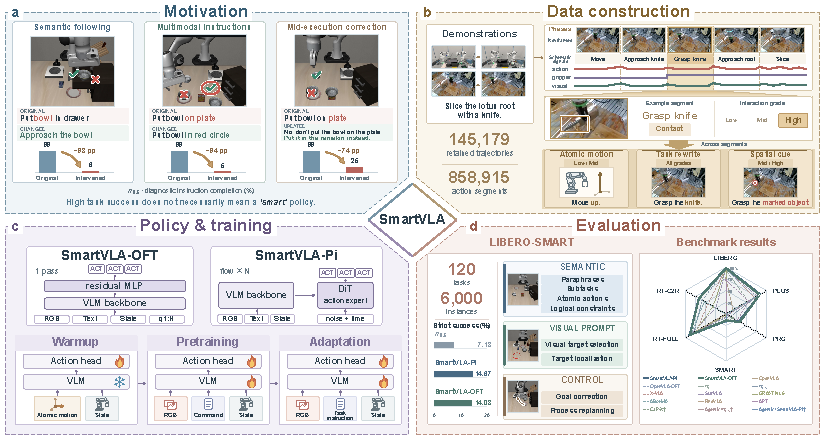
\includegraphics[width=\textwidth]{figures/fig1_overview_compact_v32.pdf}\par\nointerlineskip
  \caption{Overview of SmartVLA. (a) Behavioral diagnosis identifies failures
  in fine-grained semantic following, multimodal instruction understanding,
  and mid-execution corrective control. (b) Action-aligned data construction
  converts heterogeneous demonstrations into phase-level semantic and spatial
  supervision. (c) Warmup, pretraining, and adaptation
  train the two policies. (d) LIBERO-SMART and other
  benchmarks evaluate these three capabilities and general task performance.}
  \label{fig:overview}
\end{figure}

% Therefore, we propose \textbf{SmartVLA} to strengthen instruction-conditioned control through coordinated data construction and training看不懂后半句. Paraphrasing an entire task can increase linguistic diversity without clarifying which actions a local command should govern 没头没尾一句话，这么做结果如何. We therefore construct supervision that binds each command and visual prompt to the corresponding control phase. 

Therefore, we propose SmartVLA, a framework that combines action-aligned data construction with three-stage training to improve fine-grained semantic following, multimodal instruction understanding, and mid-execution corrective control in VLA policies. Motivated by the preceding experiment on supervision granularity, we explicitly pair local commands and visual prompts with the action segments, providing fine-grained supervision rather than relying solely on a single task-level instruction for an entire demonstration. To this end, we develop an automated \textbf{action-aligned data construction pipeline} (Figure~\ref{fig:overview}(b)): it first uses action, gripper, and visual evidence to establish segment boundaries and interaction context, then generates and reviews rewrites under grade-dependent applicability rules. This separates evidence extraction from language generation, reducing reliance on expensive end-to-end video annotation and per-segment manual rewriting while keeping instructions tied to demonstrated behavior.

Aligned supervision alone does not ensure that a policy uses language rather than visual correlations to predict actions. We therefore first establish a language-conditioned action prior, then train its realization in observed scenes, and finally adapt it to a target domain while retaining complete-task supervision. This motivates our \textbf{three-stage training recipe} (Figure~\ref{fig:overview}(c)). Warmup trains only the action head from atomic instructions and robot state, removing image-based cues while preserving the frozen backbone. Pretraining restores visual inputs and jointly trains the policy to relate local commands and visual prompts to the current scene. Adaptation mixes original-task and local supervision in the target domain, addressing the need for both complete execution and fine-grained response. The resulting interface accepts updated commands in subsequent calls, enabling human operators or upper-level models to steer ongoing behavior.


To evaluate whether these capabilities are realized in existing policies, we introduce LIBERO-SMART, which separately assesses three forms of instruction following: fine-grained semantic following, where the policy must execute the specified local action, relation, or constraint; multimodal instruction understanding, where visual prompts specify the current object or target location; and mid-execution corrective control, where the policy must adapt its subsequent actions after a command update or redirection. These capabilities are not guaranteed by success on the original task. Although $\pi_{0.5}$ achieves 96.85\% on the original LIBERO benchmark, its average success rate on LIBERO-SMART is only 7.18\%. This gap is consistent with our diagnostic observations: a policy may possess strong basic manipulation skills while failing to follow semantic requirements and visual prompts or to redirect its behavior after an intermediate command change.

On LIBERO-SMART, SmartVLA-Pi and SmartVLA-OFT achieve average success rates of 14.67\% and 14.03\%, respectively, compared with 7.18\% for $\pi_{0.5}$, with both variants outperforming all direct-policy baselines across the three suites. Ablation studies support the contributions of action-aligned segmentation, grade-conditioned rewriting, spatial supervision, and staged training to these gains. To test whether improved instruction following also benefits hierarchical robot control, we replace only $\pi_{0.5}$ with SmartVLA-Pi under a fixed upper-level protocol, raising overall system success on LIBERO-SMART from 11.83\% to 17.67\%. As summarized in Figure~\ref{fig:overview}(d), we also evaluate standard task performance on LIBERO~\citep{liu2023libero}, LIBERO-Plus~\citep{fei2025liberoplus}, LIBERO-Pro~\citep{zhou2025liberopro}, and RoboTwin~\citep{mu2025robotwin,chen2025robotwin2}, as well as real-world instruction following on the Piper platform. SmartVLA-Pi achieves 98.30\% on LIBERO and 84.00\% on LIBERO-Plus, outperforming $\pi_{0.5}$ by 1.45 and 3.74 percentage points, respectively. On Piper, it raises average success from 45.00\% to 58.50\%, a gain of 13.50 percentage points. These experiments show that SmartVLA enables smarter, more flexible, and more controllable robot behavior while maintaining strong performance on standard benchmarks.

Our contributions are:

\begin{itemize}
\item
  We develop SmartVLA to connect current instructions with local control. An action-aligned pipeline reconstructs existing demonstrations into phase-specific semantic and visual supervision, while staged training establishes a language-conditioned action prior, grounds it in observations, and adapts it to target domains with complete-task and local supervision.
\item
  We introduce LIBERO-SMART, comprising Semantic, Visual Prompt (Vis), and
  Control suites with 120 tasks and 6,000 evaluation instances across
  diverse initializations, to evaluate fine-grained semantic following,
  multimodal instruction understanding, and mid-execution corrective control.
\item
  We systematically evaluate standard task performance and the three
  instruction-following capabilities across two VLA architectures on
  the LIBERO benchmarks, RoboTwin Full and C2R, LIBERO-SMART, and the
  Piper real-robot platform. We further assess callability under a
  fixed upper-level protocol.
\end{itemize}

\hypertarget{motivating-diagnostics-why-vlas-struggle-with-diverse-instructions-and-reliable-control}{%
\section{Motivational Diagnostics}\label{motivating-diagnostics-why-vlas-struggle-with-diverse-instructions-and-reliable-control}}

The behavioral interventions reveal a gap between original-task competence and responses to local commands, visual prompts, and corrections. To determine what can be used to bridge this gap, we ask whether the relevant semantic and visual information remains accessible after action training. If it is absent, improving the mapping from existing representations to actions alone would be insufficient; the relevant representations would also need to be learned. We train target-point probes on frozen representations under paired language and visual interventions. Target assignment rates reach 83.80--98.82\%, above the 50\% two-choice reference, and predicted targets shift consistently with the interventions. These findings show that target-relevant information remains readable despite execution failures. Readability does not establish that the policy uses this information, but provides a basis for learning more explicit correspondences between current instructions, visual targets, and local actions. This motivates the supervision and training design below, rather than relying solely on additional trajectory fitting. Full protocols, metric definitions, and results are provided in Appendices~\ref{appendix:behavior-diagnostics} and~\ref{appendix:representation-diagnostics}.

\hypertarget{method}{%
\section{SmartVLA Framework}\label{method}}

\begin{figure}[t]
  \centering
  \setlength{\parskip}{0pt}
  % Match Figure 1 without negative caption or float spacing.
  \setlength{\abovecaptionskip}{\baselineskip}
  \setlength{\belowcaptionskip}{0pt}
  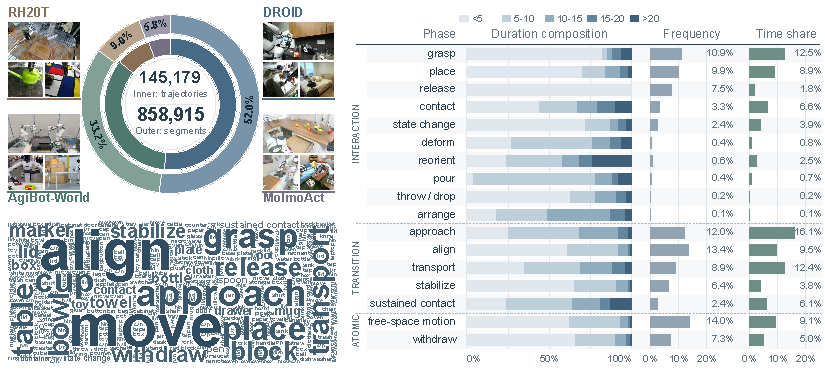
\includegraphics[width=\textwidth,trim=0 4bp 0 0,clip]{figures/fig2_data_construction_from_overleaf_20260924.pdf}\par\nointerlineskip
  \caption{SmartVLA data construction. Left: four trajectory sources,
  aligned segments, and the action vocabulary word cloud. Right:
  subtask duration composition, frequency, and total time across interaction,
  transition, and atomic-motion phases.}
  \label{fig:data-pipeline}
\end{figure}

SmartVLA builds on pretrained representations to strengthen instruction-conditioned control while retaining complete-task execution. Our diagnostics suggest a starting point: target information remains readable but does not reliably guide actions. Task-level supervision leaves this correspondence underspecified. For example, ``put the bowl on the plate'' labels approaching, grasping, transporting, and releasing without specifying the scope of ``approach the bowl'' alone. A policy may therefore use language as a task identifier and reproduce familiar actions from scene and execution cues. Whole-task paraphrases diversify descriptions without resolving this local ambiguity.

Our insight is to change the granularity of supervision--action correspondence: each command should describe a control phase, with visual prompts specifying its current object or target. Existing action changes, gripper events, and visual interactions provide evidence for these phases. Establishing behavioral scope before generating instructions turns open-ended video annotation into constrained local supervision, reducing reliance on expensive end-to-end video interpretation and per-segment manual rewriting.

Aligned data alone do not ensure that language influences action selection when visual correlations can predict familiar behavior. We therefore first learn instruction--motion correspondence without images, then ground it in observed scenes, and finally adapt to target domains while retaining complete-task supervision. The data pipeline specifies what behavior a command governs; staged training encourages the policy to use that correspondence.

\hypertarget{steering-oriented-data-construction}{%
\subsection{Action-Aligned Data Construction Pipeline}\label{steering-oriented-data-construction}}

We represent local supervision as $r_i=(\mathbf O_i,\mathbf S_i,\mathbf A_i,c_i,z_i,g_i)$: observations, robot states, and actions span a segment of length $L_i$, while $c_i$, $z_i$, and $g_i$ denote its instruction, object/target evidence, and interaction grade. Figure~\ref{fig:overview}(b) summarizes the pipeline.

\textbf{Establish behavioral scope.} Uniform cuts may split a grasp or combine distinct control phases. We instead identify boundaries from action changes, gripper events, and visual interactions, consolidate them using temporal consistency and task-family rules, and associate each segment with object and target evidence. This evidence constrains what the subsequent instruction should describe. The aim is not simply to shorten trajectories, but to align the instruction's execution scope with control-phase boundaries, reducing the inclusion of subsequent actions outside the current requirement.

\textbf{Match rewrites to interaction evidence.} We use three families: \textbf{Object-free atomic motion} specifies movement without object names; \textbf{Synonym/task rewrite} varies wording while preserving the local goal; and \textbf{Spatial visual generalization} pairs instructions with points, boxes, regions, or trajectories rendered in the observations. Low, Mid, and High grades correspond to free-space motion, transitions, and explicit object interaction. Low excludes spatial rewrites without supported targets; High excludes atomic rewrites that omit essential object relations; Mid permits all three (Table~\ref{tab:grade-policies}). For example, free-space motion such as ``move up'' need not identify an object, whereas placement must preserve what is placed and where. Grades therefore govern rewrite applicability and specificity, not segment retention.

\begingroup
% The preceding paragraph already separates this block from the text above.
% Avoid adding wrapfig's extra top inset; keep caption-to-table spacing below.
\setlength{\intextsep}{0pt}
\begin{wraptable}[10]{r}{0.38\textwidth}
\centering
\normalsize
% Keep one body-line gap between the caption and the table.
\setlength{\parskip}{0pt}
\setlength{\abovecaptionskip}{0pt}
\setlength{\belowcaptionskip}{\baselineskip}
\caption{\centering Grade-conditioned rewrite families.}
\label{tab:grade-policies}
\nointerlineskip
\setlength{\tabcolsep}{2.0pt}
\begin{tabular}{@{}lccc@{}}
\toprule
Grade & \shortstack{Atomic\\motion} & \shortstack{Synonym/\\task} & \shortstack{Spatial\\visual} \\
\midrule
Low & yes & yes & no \\
Mid & yes & yes & yes \\
High & no & yes & yes \\
\bottomrule
\end{tabular}
\end{wraptable}

\textbf{Generate and review.} The generator receives the phase, grade, and available evidence, while automated semantic and visual review filters inconsistent rewrites. Separating evidence extraction, constrained generation, and review supports scalable construction without requiring the language model to infer the entire temporal structure. Local examples form $\mathcal D_{\mathrm{local}}$; examples retaining original task instructions form $\mathcal D_{\mathrm{task}}$, preserving supervision of complete execution. Figure~\ref{fig:data-pipeline} summarizes the corpus. Appendix~\ref{appendix:data-construction} provides implementation details and illustrates the pipeline and segment-level examples in Figure~\ref{fig:appendix-action-aligned-pipeline}.

\par
\endgroup

\hypertarget{steering-centric-policy-training}{%
\subsection{Three-Stage Training Recipe}\label{steering-centric-policy-training}}

We separate learning how instructions specify motion, how observations locate its target, and how both transfer to a target domain (Figure~\ref{fig:overview}(c)). Let $\theta=(\psi,\phi)$ collect the backbone and action-head parameters. The policy predicts $\mathbf A_t=\mathbf a_{t:t+H-1}\sim\pi_\theta(\cdot\mid\mathbf o_t,\mathbf s_t,c_t)$; prediction length $H$ is distinct from segment length $L_i$. All stages retain the native per-example action loss $\ell_{\mathrm{act}}$, with objective
\begin{equation}
\label{eq:action-objective}
\mathcal L_{\mathrm{act}}(\theta;\mathcal D)=
\mathbb E_{(\mathbf o,\mathbf s,c,\mathbf A)\sim\mathcal D}
\left[\ell_{\mathrm{act}}(\theta;\mathbf o,\mathbf s,c,\mathbf A)\right].
\end{equation}

\textbf{Warmup: learn motion correspondence without image-based shortcuts.} Atomic instructions specify motion without requiring object localization. Warmup therefore receives only atomic instructions and robot state, freezes the backbone at $\psi_0$, and trains the action head with $\mathcal L_{\mathrm w}(\phi)=\mathcal L_{\mathrm{act}}((\psi_0,\phi);\mathcal D_{\mathrm{atomic}})$. Here $\mathcal D_{\mathrm{atomic}}$ contains eligible Low/Mid segments with no image input. Different atomic commands specify corresponding motion patterns, while robot state supplies the physical conditions for execution. Removing images prevents initial learning from directly relying on visual scene cues; freezing the backbone focuses optimization on how the action head uses existing representations, establishing a language-conditioned action prior for subsequent visually conditioned learning.

\textbf{Pretraining: ground the prior in current scenes.} Motion alone does not identify its target: ``lift the object in the red box'' also requires binding the prompt to the current object. Starting from warmup, we restore multi-view images and train both modules with $\mathcal L_{\mathrm p}(\theta)=\mathcal L_{\mathrm{act}}(\theta;\mathcal D_{\mathrm{mix}}^{\mathrm{pre}})$. The mixture $\mathcal D_{\mathrm{mix}}=\alpha\mathcal D_{\mathrm{task}}+(1-\alpha)\mathcal D_{\mathrm{local}}$ samples original-task and local supervision, respectively. Local commands and visual prompts teach scene-dependent control, while original-task examples retain complete-task supervision. The resulting checkpoint is SmartVLA-Base.

\textbf{Adaptation: retain both supervision granularities.} Original-task instructions alone do not preserve local command--action supervision, while local segments cannot replace supervision of complete execution. We therefore reconstruct target-domain demonstrations using Section~\ref{steering-oriented-data-construction} and independently adapt each domain $d$ from SmartVLA-Base, optimizing both modules with $\mathcal L_{\mathrm a}^{d}(\theta)=\mathcal L_{\mathrm{act}}(\theta;\mathcal D_{\mathrm{mix}}^{d})$. This continues local language and visual supervision while learning target-domain control.

SmartVLA-Pi and SmartVLA-OFT follow this recipe with their native action models. Both accept complete-task, subtask, or updated corrective commands through the same observation-conditioned interface. Architectures, initialization, sampling ratios, training settings, and the calling protocol are detailed in Appendix~\ref{appendix:model-details}.

\hypertarget{libero-smart}{%
\section{LIBERO-SMART}\label{libero-smart}}

LIBERO-Pro, LIBERO-Plus, and RoboTwin-IF evaluate generalization across changes in task goals, layouts, observations, and language requirements. Such variations are important, but robust task completion does not by itself establish that a policy follows the precise scope and execution conditions of a current instruction. For example, rephrasing ``pick up the cup and place it on the plate'' preserves the intended grasp-and-place sequence, whereas ``only approach the cup'' requires suppressing its later stages. LIBERO-SMART makes these distinctions explicit through Semantic, Visual Prompt, and Control tasks and instruction-consistent trajectory contracts (Figure~\ref{fig:overview}(d)).

\hypertarget{instruction-generalization-over-familiar-skills}{%
\subsection{Instruction Generalization over Familiar
Skills}\label{instruction-generalization-over-familiar-skills}}

The benchmark asks whether familiar manipulation capabilities can be invoked under new requirements, rather than requiring a new skill for every command. A policy that has learned grasping, transport, and placement should be able to select the requested phase, bind its target to the current observation, or redirect its continuation. We therefore retain some LIBERO scene assets and basic skills while evaluating held-out skill combinations, language conditions, object--target relations, and layouts. This separates familiar motor operations from the new conditions governing their use.

Different commands alone cannot exclude solutions based on familiar object locations. Each task therefore has 10 substantially different macro layouts and 5 local position and pose variants per layout, preserving instruction meaning and physical feasibility while changing object configurations and target locations. For Control, models start from the same intermediate physical state within each instance, so differences in preceding-stage execution do not change the difficulty of the corrective continuation.

Reaching a target also does not establish that the full instruction was followed: a policy may first manipulate a forbidden object, execute steps in the wrong order, or immediately undo the intended result. Task contracts therefore jointly assess target correctness, process constraints, and result stability, including applicable prohibitions, step-order constraints, and release or holding requirements. Together, tasks, initializations, and contracts test whether improved instruction--action correspondence yields complete instruction execution. Training--evaluation separation and detailed construction and scoring rules are provided in Appendix~\ref{appendix:smart-benchmark}.

\hypertarget{three-task-suites}{%
\subsection{Three Task Suites}\label{three-task-suites}}

LIBERO-SMART comprises three independently scored suites, Semantic,
Visual Prompt (Vis), and Control, with 40 tasks per suite and 50
initializations per task, totaling 6,000 evaluation
instances. Both direct policies and agentic systems are evaluated using
the same trajectory-level task contracts.

\textbf{Semantic.} This suite evaluates fine-grained semantic following
through requirements on the manipulated object, action scope, and
termination condition. It covers equivalent
semantic rewrites, designated subtasks of a complete episode, standalone
atomic actions, and logical constraints on object exclusivity, spatial
relations, pose, and order. For example, when an instruction only
requests picking up an object, subsequently placing it in the original
task container violates the requirement.

\textbf{Visual Prompt.} This suite evaluates multimodal instruction
understanding by testing whether models can bind explicit image cues to
the current object or spatial target. Cues include circles
identifying objects to manipulate, circles defining placement regions,
points specifying target locations, and trajectories guiding motion.
They refer to the current object or location in each initialization and
remain consistent with the language instruction and target evaluation.

\textbf{Control.} Starting from an intermediate physical state, this
suite evaluates mid-execution corrective control by testing whether
models adjust subsequent behavior according to a new instruction. Target correction changes the intended final result, for
example redirecting a held object to another target. Process re-planning
changes how subsequent actions are executed, for example holding
stably, reversing an operation, or retaining completed parts while
rearranging the remaining steps.

\hypertarget{experiments}{%
\section{Experiments}\label{experiments}}

Unless otherwise specified, SmartVLA results are reported using the corresponding target-domain-adapted experts. For LIBERO, LIBERO-Plus, LIBERO-Pro, and RoboTwin2.0, we follow the evaluation settings released with each benchmark. LIBERO-SMART task contracts and scoring are specified in Appendix~\ref{appendix:smart-benchmark}; the Piper real-robot protocol is described in Appendix~\ref{appendix:real-robot-piper}. The overall evaluation scope is summarized in Figure~\ref{fig:overview}(d). All success rates are reported as percentages.

\subsection{LIBERO-SMART}\label{libero-smart-1}

\begin{table}[htbp]
\centering
\setlength{\abovecaptionskip}{0pt}
\setlength{\belowcaptionskip}{\baselineskip}
\caption{LIBERO-SMART success rates (\%). $\dagger$ denotes an agentic system.}
\label{tab:libero-smart}
\label{tab:agentic-smart}
\nointerlineskip
\normalsize
\setlength{\tabcolsep}{3.6pt}
\begin{tabular}{@{}lrrrrr@{}}
\toprule
Method & Sem & Vis & Con & Avg. & Goal-only \\
\midrule
OpenVLA-OFT & 1.45 & 0.30 & 1.15 & 0.97 & 1.65 \\
$\pi_{0}$ & 0.00 & 0.00 & 0.00 & 0.00 & 0.85 \\
$\pi_{0.5}$ & 14.70 & 2.00 & 4.85 & 7.18 & 17.92 \\
X-VLA & 0.00 & 0.00 & 0.00 & 0.00 & 0.55 \\
GR00T N1.6 & 8.35 & 0.80 & 1.00 & 3.38 & 13.22 \\
StarVLA & 12.60 & 1.95 & 4.00 & 6.18 & 15.62 \\
CaP-X$^\dagger$ & 12.75 & 6.75 & \textbf{21.25} & 13.58 & 18.33 \\
Agentic+$\pi_{0.5}^{\dagger}$ & 17.75 & 3.50 & 14.25 & 11.83 & 18.22 \\
\midrule
\rowcolor{smartvlarow}
\textbf{SmartVLA-Pi} & 23.05 & \textbf{8.40} & 12.55 & 14.67 & 29.73 \\
\rowcolor{smartvlarow}
\textbf{SmartVLA-OFT} & 20.10 & 5.55 & 16.45 & 14.03 & 32.73 \\
\rowcolor{smartvlarow}
\textbf{Agentic+SmartVLA-Pi$^\dagger$} & \textbf{26.50} & 7.00 & 19.50 & \textbf{17.67} & \textbf{37.97} \\
\bottomrule
\end{tabular}
\end{table}

\Needspace{14\baselineskip}
\begin{wrapfigure}[14]{r}{0.51\textwidth}
\centering
\setlength{\parskip}{0pt}
\setlength{\abovecaptionskip}{\baselineskip}
\setlength{\belowcaptionskip}{0pt}
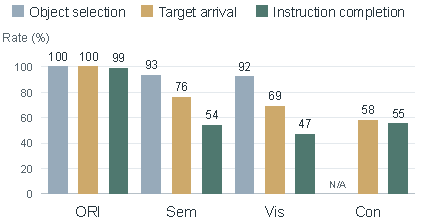
\includegraphics[width=\linewidth]{figures/fig3_behavior_diagnosis.pdf}\par\nointerlineskip
\caption{SmartVLA-Pi behavioral diagnosis (\%).}
\label{fig:smartvla-behavior}
\end{wrapfigure}

% Start the wrapped paragraph without overriding the style's line-breaking settings.
\begingroup
\leavevmode
Table~\ref{tab:libero-smart} evaluates whether SmartVLA improves the three instruction-following capabilities targeted by our method. In direct-policy evaluation, SmartVLA-Pi and SmartVLA-OFT achieve average success rates of 14.67\% and 14.03\%, compared with 7.18\% for $\pi_{0.5}$, with improvements across all three suites. The Semantic gains indicate better execution of local commands and instruction-specific constraints; the Visual Prompt gains reflect improved use of visually specified objects and target locations; and the Control gains show better adjustment to commands issued during execution. These improvements are consistent with learning segment-aligned commands and visual prompts as conditions for subsequent actions. Under Goal-only scoring, which checks any-time goal attainment without the additional contract requirements, the two variants also improve from 17.92\% for $\pi_{0.5}$ to 29.73\% and 32.73\%. Their advantage therefore extends beyond the strict scoring criterion.
\par
\endgroup

\paragraph{Behavioral diagnosis.}

Figure~\ref{fig:smartvla-behavior} revisits the motivating interventions with SmartVLA-Pi. Instruction-completion rates increase from 6.00\%, 5.00\%, and 25.00\% for $\pi_{0.5}$ to 54.00\%, 47.00\%, and 55.00\% on Semantic, Visual Prompt, and Control, respectively, while original-task completion remains at 99.00\%. This comparison connects the benchmark improvements to more reliable execution of local instructions, visual prompts, and command updates.

Under a fixed agentic protocol, replacing $\pi_{0.5}$ with SmartVLA-Pi raises strict system success from 11.83\% to 17.67\% and Goal-only success from 18.22\% to 37.97\%. Thus, improved low-level instruction following also benefits systems that invoke the policy through an upper-level controller. Calling and scoring protocols are detailed in Appendices~\ref{agentic-calling-protocol} and~\ref{app:smart-aggregation}.

\subsection{Generalization on Simulation Benchmarks}\label{simulation-benchmarks}

\paragraph{LIBERO, LIBERO-Plus, and LIBERO-Pro.}\label{libero-benchmarks}

\begin{table}[!htb]
\centering
% The float already provides the separation from the preceding text or heading.
\setlength{\abovecaptionskip}{0pt}
\setlength{\belowcaptionskip}{\baselineskip}
\caption{Success rates on LIBERO, LIBERO-Plus, and LIBERO-Pro. $\dagger$ denotes an agentic system.}
\label{tab:libero-overview}
\label{tab:libero-pro}
\normalsize
\setlength{\tabcolsep}{3.2pt}
\begin{tabular}{@{}lrrrrr@{}}
\toprule
Method & LIBERO & LIBERO-Plus & Pro-Pos. & Pro-Task & Pro-Avg. \\
\midrule
OpenVLA & 76.50 & 17.28 & 0.00 & 0.00 & 0.00 \\
OpenVLA-OFT & 97.10 & 70.02 & 5.75 & 0.63 & 3.19 \\
$\pi_{0}$ & 94.15 & 54.63 & 0.00 & 0.00 & 0.00 \\
$\pi_{0.5}$ & 96.85 & 80.26 & 20.75 & 0.75 & 10.75 \\
X-VLA & 98.05 & 70.46 & 0.75 & 6.75 & 3.75 \\
StarVLA & 96.60 & 76.08 & 4.30 & 3.90 & 4.10 \\
APT & 72.25 & 55.85 & 27.00 & 27.75 & 27.38 \\
CAP-X$^\dagger$ & -- & -- & 20.00 & 16.33 & 18.17 \\
\midrule
\rowcolor{smartvlarow}
\textbf{SmartVLA-Pi} & \textbf{98.30} & \textbf{84.00} & 30.95 & 32.35 & 31.65 \\
\rowcolor{smartvlarow}
\textbf{SmartVLA-OFT} & 98.20 & 82.76 & \textbf{31.50} & \textbf{36.10} & \textbf{33.80} \\
\bottomrule
\end{tabular}
\end{table}

Table~\ref{tab:libero-overview} examines task performance and generalization on benchmarks developed independently of LIBERO-SMART. SmartVLA-Pi and SmartVLA-OFT achieve 98.30\% and 98.20\% on LIBERO, exceeding X-VLA~\citep{zheng2025xvla} (98.05\%) while retaining strong basic manipulation performance. On LIBERO-Plus, they reach 84.00\% and 82.76\%, above $\pi_{0.5}$ (80.26\%) and APT (55.85\%). On LIBERO-Pro, both variants outperform APT on Position and Task, reaching averages of 31.65\% and 33.80\% compared with 27.38\%, while also substantially exceeding APT's original LIBERO performance of 72.25\%. These results show improved robustness to benchmark perturbations and changes in task goals and scene layouts without a loss of strong original-task performance. Detailed results are provided in Appendix~\ref{appendix:benchmark-details}.

\paragraph{RoboTwin2.0.}\label{robotwin2.0}

\begin{table}[!htb]
\centering
\setlength{\abovecaptionskip}{0pt}
\setlength{\belowcaptionskip}{\baselineskip}
\caption{RoboTwin2.0 Full and Clean2Random results. C/R denotes clean/randomized test scenes.}
\label{tab:robotwin}
\normalsize
\setlength{\tabcolsep}{2.4pt}
\begin{tabular}{@{}lrrrrrr@{}}
\toprule
Method & Full-C & Full-R & Full Avg. & C2R-C & C2R-R & C2R Avg. \\
\midrule
$\pi_{0.5}$ & 82.70 & 76.80 & 79.75 & 70.70 & 46.00 & 58.35 \\
X-VLA & 72.80 & 72.84 & 72.82 & 68.00 & 20.90 & 44.45 \\
GR00T N1.6 & 74.76 & 75.08 & 74.92 & 43.60 & 20.70 & 32.15 \\
StarVLA & 88.18 & 88.32 & 88.25 & 46.50 & 3.20 & 24.85 \\
ABot-M0 & 86.10 & 85.10 & 85.60 & 70.70 & 36.00 & 53.35 \\
FineVLA & 86.80 & 82.50 & 84.65 & -- & -- & -- \\
\midrule
\rowcolor{smartvlarow}
\textbf{SmartVLA-Pi} & \textbf{89.86} & \textbf{89.72} & \textbf{89.79} & \textbf{75.70} & 58.40 & \textbf{67.05} \\
\rowcolor{smartvlarow}
\textbf{SmartVLA-OFT} & 88.94 & 89.06 & 89.00 & 74.02 & \textbf{59.08} & 66.55 \\
\bottomrule
\end{tabular}
\end{table}

Table~\ref{tab:robotwin} extends the evaluation to bimanual manipulation. Under Full, which includes randomized scenes during adaptation, SmartVLA-Pi and SmartVLA-OFT achieve average success rates of 89.79\% and 89.00\%, exceeding StarVLA (88.25\%) and ABot-M0~\citep{yang2026abotm0} (85.60\%). Under Clean2Random, adaptation uses only clean demonstrations, yet the two variants reach averages of 67.05\% and 66.55\%, compared with 58.35\% for $\pi_{0.5}$. Their success rates on randomized test scenes reach 58.40\% and 59.08\%, respectively, versus 46.00\% for $\pi_{0.5}$, demonstrating stronger transfer to unseen scene configurations.

Together, these results show that the benefits are not confined to a benchmark explicitly designed around our three instruction-following capabilities. Improvements on independently developed task and generalization benchmarks support the broader value of aligning language and visual supervision with local actions.

\subsection{Ablation Studies}\label{ablation-studies}

\begingroup
\setlength{\parskip}{0pt}
Table~\ref{tab:ablation} examines the contributions of training stages and supervision construction. Removing warmup or pretraining, or adapting directly from the original VLM, reduces performance, supporting the three-stage procedure. Adaptation using only original demonstrations also degrades performance, indicating that local instruction supervision remains important in the target domain.

\Needspace{18\baselineskip}
\begin{wraptable}{r}{0.54\textwidth}
\centering
\setlength{\abovecaptionskip}{0pt}
\setlength{\belowcaptionskip}{\baselineskip}
\caption{\centering SmartVLA-Pi ablations on \mbox{LIBERO-SMART} (\%).}
\label{tab:ablation}
\normalsize
\setlength{\tabcolsep}{3pt}
\begin{tabular}{@{}lrrrr@{}}
\toprule
Setting & Sem & Vis & Con & Avg. \\
\midrule
w/o warmup & 19.70 & 7.35 & 11.15 & 12.73 \\
w/o pretraining & 13.90 & 2.55 & 5.10 & 7.18 \\
From raw VLM & 14.05 & 2.30 & 4.80 & 7.05 \\
Raw-data adaptation & 16.85 & 4.25 & 5.10 & 8.73 \\
Uniform segmentation & 12.20 & 5.55 & 4.60 & 7.45 \\
w/o grade conditioning & 20.40 & 6.30 & 10.05 & 12.25 \\
Fine-grained sem. only & 15.10 & 2.05 & 3.85 & 7.00 \\
\midrule
\rowcolor{smartvlarow}
\textbf{Full SmartVLA-Pi} & \textbf{23.05} & \textbf{8.40} & \textbf{12.55} & \textbf{14.67} \\
\bottomrule
\end{tabular}
\end{wraptable}

Uniform temporal segmentation reduces average success from 14.67\% to 7.45\%, supporting alignment with control phases rather than merely annotating shorter trajectories. Removing grade conditioning further weakens performance. The FineVLA-inspired fine-grained semantic-only setting reaches 7.00\%, indicating that enriching whole-trajectory language alone does not recover the benefits of the full construction. These comparisons support the roles of action-aligned segmentation, phase-appropriate rewriting, and staged training; setting definitions are provided in Appendix~\ref{appendix:ablation-details}.
\par
\endgroup

\subsection{Real-Robot Piper Evaluation}\label{real-robot-piper-evaluation}

\Needspace{12\baselineskip}
\begin{wrapfigure}[12]{r}{0.60\textwidth}
\centering
\setlength{\parskip}{0pt}
\setlength{\abovecaptionskip}{\baselineskip}
\setlength{\belowcaptionskip}{0pt}
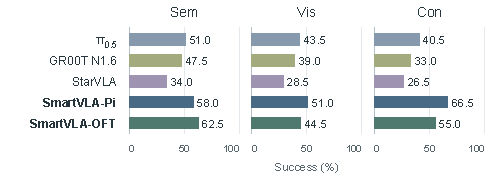
\includegraphics[width=\linewidth]{figures/fig4_piper_results.pdf}\par\nointerlineskip
\caption{Real-robot instruction following on Piper (\%).}
\label{fig:piper-results}
\end{wrapfigure}

% Retain the style's line-breaking settings in the wrapped paragraph.
\begingroup
\leavevmode
Beyond simulation, we evaluate fine-grained semantic following, multimodal instruction understanding, and mid-execution corrective control on a bimanual Piper platform.
Each category contains
10 tasks, with 20 trials per task, for a total of 600 trials per model. The
tasks build on basic operations such as grasping, placing, moving, and
holding, varying language requirements, visual targets, or commands during
execution to test whether policies adjust their behavior to the current
instruction. Models use matched tasks, initial conditions, and interaction
budgets, with results reported separately for the three capabilities in
Figure~\ref{fig:piper-results}. Representative execution
trajectories are provided in Appendix~\ref{appendix:real-robot-piper}.
\par
\endgroup

In the bimanual Piper evaluation, SmartVLA-Pi and SmartVLA-OFT achieve
average success rates of 58.50\% and 54.00\%, respectively, exceeding
the strongest baseline, $\pi_{0.5}$ (45.00\%), by 13.50 and 9.00 percentage
points. On Semantic, Visual Prompt, and Control, the best result across
the two variants exceeds $\pi_{0.5}$ by 11.50, 7.50, and 26.00 percentage
points, respectively. These results show that SmartVLA also improves
fine-grained semantic following, multimodal instruction understanding,
and mid-execution corrective control in real-robot manipulation, rather
than only improving performance on simulation benchmarks.

\hypertarget{conclusion}{%
\section{Conclusion}\label{conclusion}}

We present SmartVLA, a framework for training and evaluating VLA policies
beyond task-level control. Behavioral and representation diagnostics reveal
that decodable target information does not necessarily lead to actions
consistent with the current instruction. To address this gap, SmartVLA
combines action-aligned semantic and spatial supervision with three-stage
training, improving fine-grained semantic following, multimodal instruction
understanding, and mid-execution corrective control. We further introduce LIBERO-SMART, which
uses diverse initializations and trajectory-level task contracts to
assess complete instruction following rather than target attainment
alone. Simulation and real-robot experiments with two policy
architectures show that SmartVLA improves instruction following and
generalization while maintaining strong basic task performance. These
results support fine-grained instruction supervision aligned with action
segments as an effective approach to improving VLA steerability, enabling
the same policy to support natural human-robot interaction and serve as a
flexibly callable control interface in hierarchical robotic systems.

\section*{AI Use Statement}
We used AI tools in the dataset-construction pipeline to propose candidate
segment-level annotations and language/spatial rewrites under predefined
rules, review their semantic and visual consistency, and filter the
resulting records. The authors remain responsible for the final dataset and its use.
We also used language-model
assistance for translation, grammar
editing, and document formatting. AI was not used to generate experimental
results, determine evaluation outcomes, or make the final scientific claims;
all technical claims, methods,
experimental settings, numerical results, and interpretations are the
responsibility of the authors and have been independently verified by the authors.

\section*{Reproducibility Statement}
To support reproducibility, we will release
after publication the source code for data processing, annotation,
training, inference, and evaluation, together with the SmartVLA model
checkpoints. We will also release the LIBERO-SMART task definitions,
initialization files, evaluators, associated configurations, and
documentation needed to reproduce the reported experiments.

\bibliographystyle{iclr2027_conference}
\bibliography{paper}

\clearpage
\appendix
\section*{Appendix}

\hypertarget{related-work}{%
\section{Related Work}\label{related-work}}

\hypertarget{generalist-vision-language-action-policies}{%
\subsection{Generalist Vision-Language-Action
Policies}\label{generalist-vision-language-action-policies}}

Generalist VLA models combine the semantic understanding capabilities of vision-language models with robot control, improving task execution and generalization through advances in backbones, data scale, and action modeling. The RT family demonstrates the scalability of language-conditioned policies trained on large-scale robot data~\citep{brohan2022rt,brohan2023rt,openx2023embodiment}, while OpenVLA integrates an open VLM backbone with robot action prediction~\citep{kim2024openvla,kim2025fine}. Building on a flow-matching action expert, the $\pi$ family combines heterogeneous robot data, high-level semantic prediction, and multimodal co-training to improve the open-world generalization and steerability of continuous-action policies~\citep{black2024pi,intelligence2025pi,intelligence2025pi06,intelligence2026pi07}. VLA work in the Qwen family explores unified alignment of multi-source robot data at the representation, action, and behavior levels, as well as the role of data scale and alignment quality in generalization across environments, embodiments, and instructions~\citep{wang2026qwenvla,yuan2026qwenrobotmanip}. However, task execution and generalization performance under task-level instructions do not directly establish whether a policy can reliably translate local commands, explicit spatial cues, and requirements updated during execution into subsequent actions. SmartVLA complements these efforts without introducing a new backbone architecture. Instead, it combines action-aligned data construction with staged training to transform existing robot trajectories into semantic and spatial supervision aligned with local control phases, learning a mapping from current instructions to local actions that supports fine-grained instruction following, responses to spatial cues, and steering during execution.

\hypertarget{agentic-harnesses-and-callable-vla-interfaces}{%
\subsection{Agentic Harnesses and Callable VLA
Interfaces}\label{agentic-harnesses-and-callable-vla-interfaces}}

Recent agentic robotic systems organize execution as a closed loop linking high-level reasoning and orchestration with low-level skill invocation. Works such as CaP-X~\citep{fu2026capx}, ASPIRE~\citep{lu2026aspire}, and Zetta~\citep{ding2026zetta} improve task decomposition, memory, tool use, and failure handling through code-based policies, skill libraries and search, and runtime critique and recovery. Stronger general-purpose multimodal models such as GPT-6 Astra~\citep{openai2026gpt6astra} further advance long-horizon reasoning, visual state understanding, tool use, and dynamic replanning, enabling high-level harnesses to continuously orchestrate low-level skills based on current observations and execution feedback. However, stronger high-level reasoning and orchestration do not automatically ensure that low-level policies reliably follow updated commands and satisfy spatial requirements. SmartVLA complements these efforts: the high-level harness handles subgoal generation, skill selection, and plan revision, while SmartVLA uses the current command, visual cues, and robot state to translate semantic and spatial requirements into local actions and respond to updated instructions in subsequent calls. We compare policies under a fixed high-level harness, replacing only the low-level VLA, to assess how low-level instruction execution affects system performance without attributing gains from high-level planning, prompt engineering, or tool selection to the low-level policy.

\hypertarget{steerable-and-instruction-generalizable-policies}{%
\subsection{Steerable and Instruction-Generalizable
Policies}\label{steerable-and-instruction-generalizable-policies}}

Another line of work focuses on fine-grained language, steerability, and instruction generalization. FineVLA~\citep{hu2026finevla} uses fine-grained language supervision to provide execution-critical details, while Steerable Policies~\citep{chen2026steerable} enables low-level policies to be invoked through subtask commands. APT~\citep{xu2026apt} and BeTTER~\citep{xu2026better} investigate issues such as sparse language supervision, visual shortcuts, vocabulary-motion associations, and behavioral inertia through action-expert pretraining and spatial-layout and temporal interventions, respectively. These works collectively emphasize that final task success rates alone cannot establish whether the current instruction actually constrains action execution. Following this direction, we focus on aligning semantic and spatial supervision with local actions, using data construction and training to improve policy responsiveness to fine-grained instructions, explicit spatial cues, and instruction updates during execution.

\section{Behavioral Intervention Diagnosis Protocol}
\label{appendix:behavior-diagnostics}

\subsection{Condition Construction and Instance Pairing}

We evaluate $\pi_{0.5}$, GR00T N1.6, and StarVLA under four conditions:
ORI, Semantic (Sem), Visual Prompt (Vis), and Control (Con). ORI retains the original task instruction and scene to
measure basic task execution. Semantic keeps the scene and task context
executable while changing the object, local action, target relation, or
holding/termination requirement. Vis changes object or target layout,
or adds a circle, point, region, or trajectory in the image as the visual
target. Control starts from an intermediate state in which the robot holds
the object and replaces the target or subsequent process requirement.
The initial held state in Control is not counted as a new object
selection.

The three models use the same instances, environment initializations, and
intervention commands. Each model is evaluated on 100 instances per
condition, for 1,200 rollouts in total. Semantic commands cover phase
sub-tasks, atomic motions, object roles, spatial relations, and holding or
termination requirements. Visual prompts are synchronized with the current
object or target region, and Control commands are applied only to
physically executable intermediate states. For each rollout, we record the original
task, initialization, intervention command, and applicable evaluation conditions.

\subsection{Behavioral Metrics}

We report three binary metrics:

\begin{itemize}
\item
  \textbf{Target-object selection rate}: the specified object is correctly
  grasped at least once during execution. This metric is not applicable
  to Control, which starts with an object already held.
\item
  \textbf{Target-position attainment rate}: the manipulated object reaches
  the position, region, or target relation specified by the current
  instruction at least once.
\item
  \textbf{Instruction-completion rate}: all applicable relational,
  sequential, release, holding, and termination requirements are
  satisfied.
\end{itemize}

Correct object selection or transient target attainment does not imply
complete execution. These metrics decompose the behavioral chain and do
not replace the LIBERO-SMART trajectory contract or define a ranking
across architectures.

\subsection{Trajectory Review}

Behavior is judged jointly from state trajectories, action trajectories,
and task conditions. Representative rollouts are reviewed frame by frame
to determine whether the correct object was selected, whether the target
changed with the current condition, whether the obsolete task continued,
and whether unnecessary actions occurred after a local goal was reached.
The main recurring failure patterns are summarized in
Table~\ref{tab:behavior-failure-patterns} and illustrated in
Figure~\ref{fig:behavior-examples}. The complete quantitative
metrics are reported in Appendix~\ref{appendix:representation-diagnostics}, Table~\ref{tab:diagnostics}.

\subsection{Behavioral Results and Failure Patterns}
\label{behavioral-diagnosis}

All three models correctly select the object and reach the original target under ORI, with complete-task success rates of 96--99\%. Under Sem, target-object selection remains at 79--88\%, but target-position attainment drops to 3--11\%, and instruction completion falls to only 1--6\%. Correctly identifying and grasping the object therefore does not ensure that the subsequent execution satisfies the specified local action, target relation, or holding and termination requirements.

Under Vis, target-object selection remains at 72--83\%, while target-position attainment is only 3--14\% and instruction completion is only 2--5\%. Under Con, target-position attainment and instruction completion range from 6\% to 25\%, despite starting from a physically executable state with the object already held. These results distinguish object selection, target-position attainment, and complete instruction execution: success at an earlier part of the behavior does not guarantee that subsequent actions satisfy the current instruction. Table~\ref{tab:diagnostics} reports the full results.

\begin{center}
\setlength{\belowcaptionskip}{\baselineskip}
\captionof{table}{Recurring behavior patterns observed in trajectory review.}
\label{tab:behavior-failure-patterns}
\normalsize
\setlength{\tabcolsep}{3.5pt}
\begin{tabular}{@{}lll@{}}
\toprule
Pattern & Observable behavior & Capability gap \\
\midrule
Target carryover & Correct grasp, original target retained & Target rebinding \\
Visual-target decoupling & Placement not bound to the visual cue & Visual-prompt grounding \\
Command inertia & Old sequence continues after update & Mid-execution correction \\
Unrequested continuation & Grasp followed by unwanted placement & Termination and holding \\
\bottomrule
\end{tabular}
\end{center}

Figure~\ref{fig:behavior-examples} compares $\pi_{0.5}$ and SmartVLA on four
diagnostic tasks, highlighting whether execution follows the instructed
object--target relation, visual prompt, updated destination, or holding
requirement.

\begin{figure}[!htbp]
  \centering
  \setlength{\parskip}{0pt}
  \setlength{\abovecaptionskip}{\baselineskip}
  \setlength{\belowcaptionskip}{0pt}
  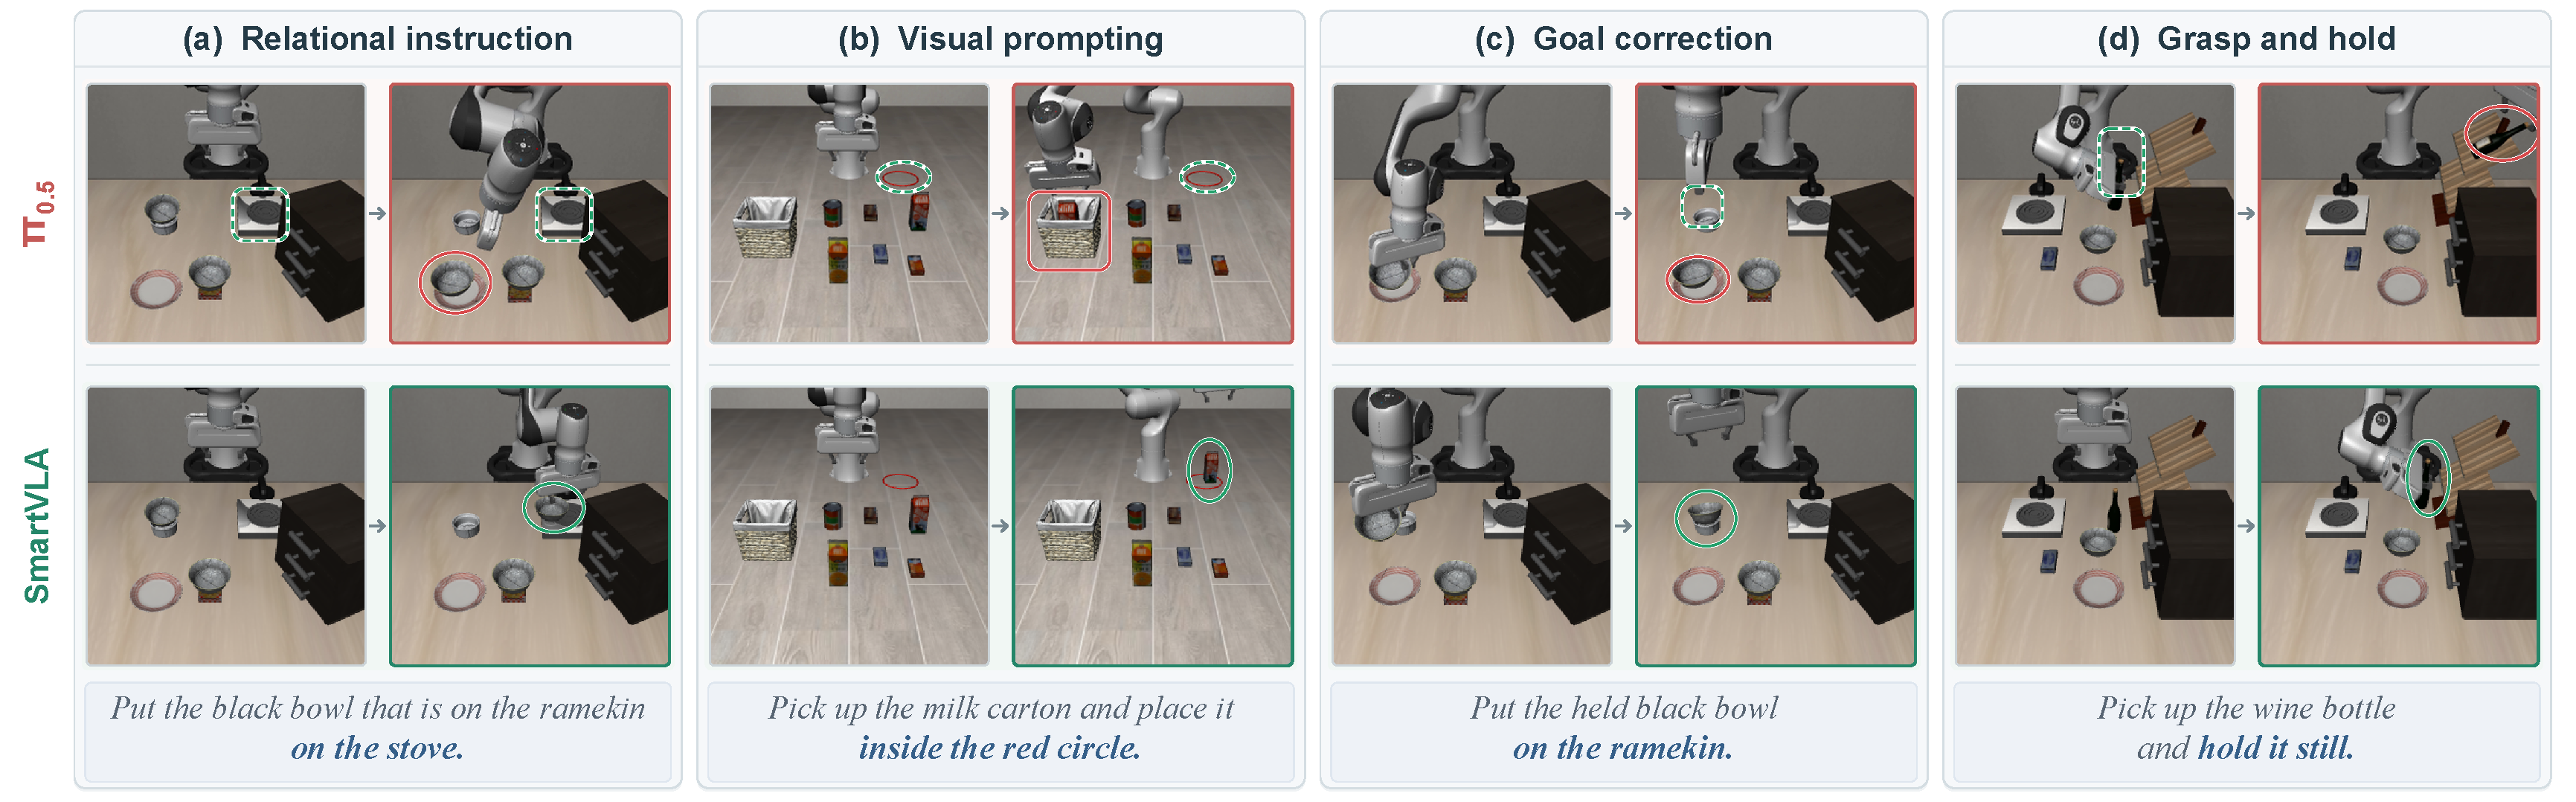
\includegraphics[width=\textwidth]{fig_behavior_comparison_v5.pdf}\par\nointerlineskip
  \caption{Qualitative comparison of $\pi_{0.5}$ (upper row) and SmartVLA
  (lower row) under the same diagnostic instructions. Instructions appear
  below each column; paired frames progress from left to right.
  (a) Relational instruction: placing the specified bowl on the stove
  rather than the plate. (b) Visual prompting: placing the milk inside the
  red circle rather than the basket. (c) Goal correction: redirecting the
  held bowl to the ramekin rather than the plate. (d) Grasp and hold:
  keeping the wine bottle grasped rather than continuing to place it on
  the rack. $\pi_{0.5}$ continues toward an unintended placement target, whereas
  SmartVLA follows the requested destination or holding condition.}
  \label{fig:behavior-examples}
  \label{fig:behavior-success-examples}
\end{figure}

\section{Representation Probe Diagnosis Protocol}
\label{appendix:representation-diagnostics}

\subsection{Probe Setup and Paired Interventions}

The probes test whether failures of instruction following coexist with accessible target information in the action-trained representations. If this information is absent, strengthening its correspondence with actions alone cannot exploit an existing semantic representation. Conversely, reliable decoding motivates supervision that links the available information to the required behavior. The probes measure accessibility in the final frozen policies, rather than changes from their original VLMs or the causal contribution of an individual action head.

We freeze $\pi_{0.5}$, GR00T N1.6, and StarVLA and train a common-form
conditional target-point probe over each model's multimodal fusion
representation. The probe receives language and visual representations
associated with the current command and predicts a two-dimensional target
point. Behavior and probe results use the same paired instances.

Sem switches fine-grained commands while holding image and robot state
fixed, testing whether the target representation changes with semantics.
Vis changes scene layout or moves an explicit visual cue, testing whether
the representation binds to the current visual position. Con switches
target commands in an action-contrast subset, testing whether the internal
target representation updates with the control requirement. Sem uses
fine-grained commands from the original task templates, Vis uses explicit
visual targets under a unified protocol, and Con uses paired commands in
the action-contrast subset.

All three models use matched instance pairs, target annotations, and probe-training
budgets; the feature location is selected at the corresponding multimodal
fusion layer.

\subsection{Representation Metrics}

Let $\hat{\mathbf{x}}$ be the predicted target point, $\mathbf{x}$ the
current target, and $\mathbf{x}'$ the alternative candidate, expressed in
the same evaluation-image coordinate system. The per-instance target-point
error is $e=\lVert\hat{\mathbf{x}}-\mathbf{x}\rVert_2$ in pixels. Target
assignment measures the proportion of predictions satisfying
$\lVert\hat{\mathbf{x}}-\mathbf{x}\rVert_2 <
\lVert\hat{\mathbf{x}}-\mathbf{x}'\rVert_2$; its two-choice reference is
50\%, and it is distinct from behavioral object selection or task completion.
Representation response direction measures agreement between the change
in predicted target position and the true target displacement across a
paired language or visual intervention.

These metrics measure the readability of target information in frozen
representations and its response to interventions. They do not directly
measure whether actions follow that information and are therefore
interpreted jointly with the behavioral results in Appendix~\ref{behavioral-diagnosis}.

\subsection{Results and Interpretation}
\label{representation-diagnosis}

\Needspace{0.28\textheight}
\begin{center}
\setlength{\belowcaptionskip}{\baselineskip}
\captionof{table}{Behavioral and representation diagnostics for $\pi_{0.5}$, GR00T
N1.6, and StarVLA. Obj., Pos., and Comp. are behavioral rates (\%), Err. is
target-point error in pixels, Assign. is target assignment (\%), and Resp. is
representation response direction.}
\label{tab:diagnostics}
\normalsize
\setlength{\tabcolsep}{4pt}
\renewcommand{\arraystretch}{1.10}
\begin{tabular}{@{}llrrrrrr@{}}
\toprule
Model & Cond. & Obj.$\uparrow$ & Pos.$\uparrow$ & Comp.$\uparrow$ &
Err.$\downarrow$ & Assign.$\uparrow$ & Resp.$\uparrow$ \\
\midrule
$\pi_{0.5}$ & ORI & 100.00 & 100.00 & 99.00 & -- & -- & -- \\
$\pi_{0.5}$ & Sem & 88.00 & 11.00 & 6.00 & 14.19 & 96.63 & 0.927 \\
$\pi_{0.5}$ & Vis & 83.00 & 14.00 & 5.00 & 20.26 & 91.09 & 0.873 \\
$\pi_{0.5}$ & Con & -- & 25.00 & 25.00 & 12.02 & 97.50 & 0.978 \\
GR00T N1.6 & ORI & 100.00 & 100.00 & 98.00 & -- & -- & -- \\
GR00T N1.6 & Sem & 79.00 & 5.00 & 1.00 & 12.26 & 96.72 & 0.967 \\
GR00T N1.6 & Vis & 80.00 & 3.00 & 2.00 & 18.35 & 92.11 & 0.896 \\
GR00T N1.6 & Con & -- & 13.00 & 11.00 & 16.18 & 93.89 & 0.912 \\
StarVLA & ORI & 100.00 & 100.00 & 96.00 & -- & -- & -- \\
StarVLA & Sem & 86.00 & 3.00 & 2.00 & 11.93 & 98.82 & 0.981 \\
StarVLA & Vis & 72.00 & 9.00 & 4.00 & 23.14 & 83.80 & 0.832 \\
StarVLA & Con & -- & 6.00 & 6.00 & 19.66 & 89.64 & 0.877 \\
\bottomrule
\end{tabular}
\end{center}

Table~\ref{tab:diagnostics} reports the paired behavioral and representation diagnostics. Target assignment rates are 96.63--98.82\% under Sem, 83.80--92.11\% under Vis, and 89.64--97.50\% under Con, all above the 50\% two-choice reference. The corresponding response-direction scores are 0.927--0.981, 0.832--0.896, and 0.877--0.978. These results indicate that the frozen representations retain decodable target information that varies with fine-grained commands, explicit visual prompts, and updated control requirements.

However, decodability does not imply that the policy effectively uses this information to generate actions. The low behavioral completion rates, despite positive target-assignment and response-direction results, reveal a gap between target information in the representations and execution that follows the current instruction. This contrast supports action-aligned supervision connecting current instructions and visual prompts to local actions, but does not by itself establish complete instruction understanding or identify a unique cause of execution failure.

\section{Data Construction and Annotation Details}
\label{appendix:data-construction}

This appendix details the data construction method in Section~\ref{steering-oriented-data-construction},
including data sources, quality filtering and unified representations,
action-first segmentation, grade-conditioned annotation, instruction
rewriting, and exported data statistics.

\hypertarget{raw-trajectory-sources}{%
\subsection{Raw Trajectory Sources}\label{raw-trajectory-sources}}

The raw trajectory pool consists of DROID~\citep{khazatsky2024droid},
MolmoAct~\citep{lee2025molmoact}, AgiBot-World~\citep{agibot2025world}, and
RH20T~\citep{fang2023rh20t}. DROID contains large-scale single-arm Franka teleoperation data
collected across real scenes, with 76K trajectories, 564
scenes, and 86 tasks. MolmoAct contains 10,689 high-quality single-arm
Franka trajectories over 93 household and tabletop tasks. AgiBot-World
provides million-scale real-robot data, including
1,001,552 trajectories, 217 tasks, and 87 skill
categories. RH20T contains more than 110K contact-rich robot
manipulation sequences with human-operation videos or demonstrations;
its task collection comprises 147 tasks. Table~\ref{tab:raw-sources} reports the complete public scale of each
dataset, not the number retained or segmented by SmartVLA; those counts
are reported separately below.

\begingroup
\normalsize
\setlength{\tabcolsep}{4pt}
\setlength{\LTcapwidth}{\linewidth}
\setlength{\LTpre}{\baselineskip}
\setlength{\LTpost}{\baselineskip}
\renewcommand{\arraystretch}{1.10}
\begin{longtable}[]{@{}
  >{\raggedright\arraybackslash}p{(\columnwidth - 6\tabcolsep) * \real{0.18}}
  >{\raggedleft\arraybackslash}p{(\columnwidth - 6\tabcolsep) * \real{0.25}}
  >{\raggedleft\arraybackslash}p{(\columnwidth - 6\tabcolsep) * \real{0.15}}
  >{\raggedright\arraybackslash}p{(\columnwidth - 6\tabcolsep) * \real{0.42}}@{}}
\caption{Public raw trajectory sources used to construct the training pool.}\label{tab:raw-sources}\\
\toprule\noalign{}
\begin{minipage}[b]{\linewidth}\raggedright
Dataset
\end{minipage} & \begin{minipage}[b]{\linewidth}\raggedleft
Public raw trajectories / sequences
\end{minipage} & \begin{minipage}[b]{\linewidth}\raggedleft
Tasks
\end{minipage} & \begin{minipage}[b]{\linewidth}\raggedright
Collection coverage
\end{minipage} \\
\midrule\noalign{}
\endhead
\bottomrule\noalign{}
\endlastfoot
DROID & 76K & 86 tasks & 564 scenes; single-arm Franka \\
MolmoAct & 10k & 93 tasks & home and tabletop; single-arm
Franka \\
AgiBot-World & 1,001k & 217 tasks & 106
scenes; 100 real robots \\
RH20T & 110K & 147 tasks & 7 configurations
across 4 robot types \\
\end{longtable}
\endgroup

\hypertarget{pipeline-overview}{%
\subsection{Pipeline Overview}\label{pipeline-overview}}

The SmartVLA pipeline decomposes the conversion from raw trajectories to
trainable steering supervision into seven stages. We first filter and
canonicalize data across sources, then use action and visual evidence to
determine boundaries, object locations, and spatial cues, and finally
generate replaceable instruction rewrites. The complete stage mapping is
shown in Table~\ref{tab:pipeline}.

The pipeline separates trajectory analysis, instruction generation, and consistency review. Action and visual evidence first define segment records containing control phases, object roles, and spatial candidates. Grade-conditioned rules then restrict instruction generation to descriptions appropriate for those records, and the review stage removes inconsistent language or spatial labels. This organization reuses existing demonstrations and grounds language generation in structured evidence, rather than requiring unconstrained descriptions to determine the full temporal structure.

Figure~\ref{fig:appendix-action-aligned-pipeline} illustrates these operations
using an RH20T demonstration of slicing lotus root with a knife. The
segment-level examples show how one task yields distinct local requirements:
approaching and grasping the knife, transferring and aligning it, slicing,
and withdrawing. Each segment receives applicable language rewrites and
visual prompts tied to its behavior and target, rather than inheriting the
same complete-task description. High-interaction segments retain task and
visual-prompt rewrites without object-free atomic-motion variants.

\begin{figure}[!t]
\centering
\setlength{\parskip}{0pt}
\setlength{\abovecaptionskip}{\baselineskip}
\setlength{\belowcaptionskip}{0pt}
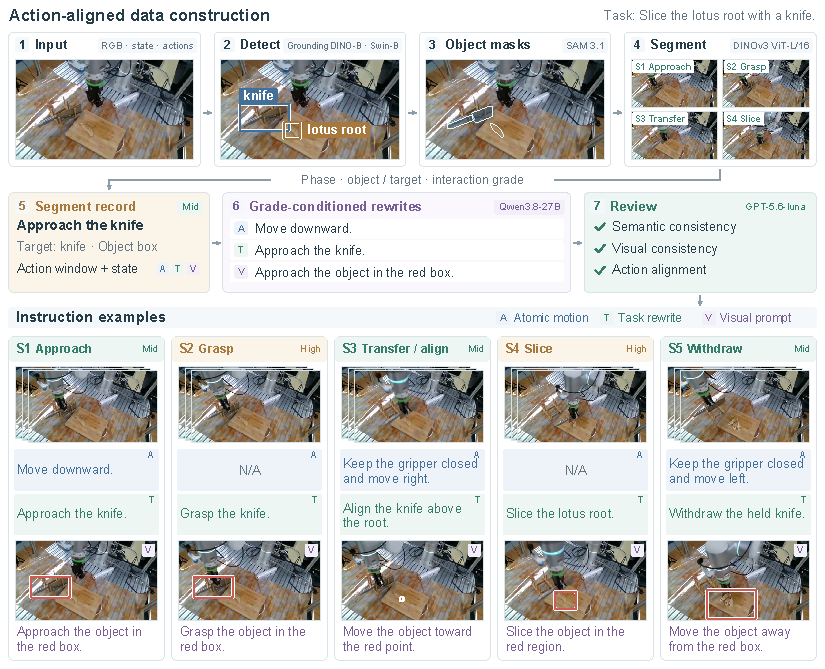
\includegraphics[width=\textwidth]{figures/appendix_action_aligned_pipeline_v12.pdf}\par\nointerlineskip
\caption{Action-aligned data construction illustrated with an RH20T
knife-and-lotus-root demonstration. Top: visual evidence extraction,
action-aligned segmentation, segment recording, grade-conditioned rewriting,
and consistency review. Bottom: atomic-motion (A), task-language (T), and
visual-prompt (V) examples for approach, grasp, transfer/alignment, slicing,
and withdrawal. N/A indicates that atomic-motion rewriting is excluded for
High-interaction segments.}
\label{fig:appendix-action-aligned-pipeline}
\end{figure}

\begingroup
\normalsize
\setlength{\tabcolsep}{4pt}
\setlength{\LTcapwidth}{\linewidth}
\setlength{\LTpre}{\baselineskip}
\setlength{\LTpost}{\baselineskip}
\renewcommand{\arraystretch}{1.10}
\begin{longtable}[]{@{}
  >{\raggedright\arraybackslash}p{(\columnwidth - 6\tabcolsep) * \real{0.20}}
  >{\raggedright\arraybackslash}p{(\columnwidth - 6\tabcolsep) * \real{0.28}}
  >{\raggedright\arraybackslash}p{(\columnwidth - 6\tabcolsep) * \real{0.32}}
  >{\raggedright\arraybackslash}p{(\columnwidth - 6\tabcolsep) * \real{0.20}}@{}}
\caption{Seven-stage steering-oriented data construction pipeline.}\label{tab:pipeline}\\
\toprule\noalign{}
\begin{minipage}[b]{\linewidth}\raggedright
Stage
\end{minipage} & \begin{minipage}[b]{\linewidth}\raggedright
Main evidence
\end{minipage} & \begin{minipage}[b]{\linewidth}\raggedright
Operation
\end{minipage} & \begin{minipage}[b]{\linewidth}\raggedright
Output
\end{minipage} \\
\midrule\noalign{}
\endfirsthead
\toprule
Stage & Main evidence & Operation & Output \\
\midrule
\endhead
\bottomrule\noalign{}
\endlastfoot
A. Filtering and normalization & language labels, video decodability,
image quality, state/action statistics & remove unlabeled, low-quality,
or noisy samples and unify image, state, and action formats & valid
trajectories in a canonical format \\
\midrule
B. Candidate boundary generation & action increments, action curvature,
gripper events, visual changes, detection and segmentation & extract
candidate peaks from action/visual curves and merge overly short
segments by temporal smoothing & candidate control segments \\
\midrule
C. Interaction evidence modeling & object masks and tracks,
gripper-to-target distance, contact evidence, object motion, gripper
state & infer active object, target region, contact relation, and
control relevance & interaction curves and spatial candidates \\
\midrule
D. Action-first refinement & intermediate records from B/C, task-family
priors, action segments & refine boundaries, assign a segment grade, and
bind semantic actions to object relations & action-aligned segment
records \\
\midrule
E. Grade-conditioned rewriting & segment grade, original task, action
primitive, object/target roles, visual/spatial evidence & select
applicable rewrite families by grade and generate candidates &
grade-organized rewrite pool \\
\midrule
F. Rewrite sampling metadata & task type, phase, rewrite family, segment
grade & record recommended sampling weights and applicability conditions
& typed rewrite pool with sampling metadata \\
\midrule
G. VLM review and expansion & keyframes, rewrite candidates, spatial
candidates & review spatial cues and language rewrites, add constrained
expressions, and disable unreliable labels & reviewed segment
annotations \\
\end{longtable}
\endgroup

This decomposition exposes auditable intermediate products. Incoming
trajectories pass language, image, action-quality, and canonical-schema
checks; boundaries come from action and visual curves; spatial cues come
from detection, segmentation, tracking, motion, and contact evidence;
and rewrites come from constrained segment records. The final output is
not a single caption but two complementary forms of supervision: one
describes phase sub-tasks, atomic motions, object roles, and relational
constraints, while the other encodes visible targets, regions, and
motion trajectories as multimodal inputs. Every training example can be
traced to a source segment, interaction evidence, and rewrite type.

\hypertarget{filtering-and-canonical-normalization}{%
\subsection{Filtering and Canonical
Normalization}\label{filtering-and-canonical-normalization}}

We first perform quality filtering. We remove three categories of
unlearnable or highly noisy samples. First, episodes or spans without
language labels or with empty task text cannot provide a stable
instruction anchor. Second, we remove poor visual data, including
undecodable videos, black or corrupted frames, severe blur, missing key
views, camera jumps, and targets that remain invisible for an extended
period. Third, we remove poor actions, including missing state/action
values, NaNs or out-of-range actions, long idle periods, clear
video-action desynchronization, failed initialization, abnormal gripper
state, and trajectories that are too short.

After filtering, action-first segmentation processes only trajectories
with readable task language, usable visual observations, and learnable
action signals. We map each source to a common multimodal control
format. Every sample contains a third-person view and the wrist view of
the currently active arm: single-arm trajectories retain one wrist view,
while bimanual trajectories retain left and right wrist views
separately; side and auxiliary views are retained when available.

To support both single-arm and bimanual embodiments, we use fixed
32-dimensional state and action containers and record embodiment type,
active arm, and a valid-dimension mask for every sample. Single-arm data
occupies one arm slot. Bimanual data such as AgiBot-World writes the
left and right arm state/action into independent slots. Each arm slot
primarily represents end-effector pose, gripper state, and relative
end-effector action. Base, waist, joint, force, and other information is
stored in reserved dimensions or retained as auxiliary proprioception.
Padding dimensions unused by the current embodiment do not contribute to
the training loss.

Action normalization is also performed at this stage. We prioritize
available end-effector poses, Cartesian actions, or end-effector poses
reliably computed by forward kinematics. Absolute end-effector targets
are converted into increments relative to the current state, while
native end-effector increments retain their control semantics and are
reordered into a common axis convention. Normalization statistics are
computed per data source and embodiment configuration over valid state
and action dimensions, including means, standard deviations, quantiles,
and clipping ranges. Different sources therefore share tensor interfaces
and dimension semantics while retaining the true scale and control
distribution of each robot.

\hypertarget{action-first-segmentation}{%
\subsection{Action-First Segmentation}\label{action-first-segmentation}}

SmartVLA derives segment boundaries from action and visual evidence
rather than free-form descriptions from a language model. We compute
adjacent action-vector differences, action curvature, gripper
opening/closing events, embedding shifts in third-person and wrist
views, and changes in open-vocabulary object observations. Candidate
boundaries are merged into segments using temporal smoothing and
task-family rules. This aligns each action segment with a local control
phase, rather than binding an episode-level caption to every timestep.

We use DINOv3 ViT-L/16 to compute cross-frame visual changes,
GroundingDINO-B with a Swin-B backbone to localize candidate objects in
keyframes, and SAM~3.1 to obtain object or target-region masks.
Point/box trackers and temporal consistency checks propagate locations
through the trajectory. Because the detector requires text queries, we
extract names of manipulated and target objects from the original
instruction and augment them with descriptions implied by the candidate
segment phase. We then combine gripper-to-target distance, contact
evidence, object motion, and gripper state to infer the active object,
target region, and interaction phase for each segment.

The resulting action segments provide local steering supervision,
while original-task examples retain their continuous
demonstration trajectories. Unused embodiment dimensions remain masked as
described above.

\hypertarget{grade-conditioned-steering-instruction-rewriting}{%
\subsection{Grade-Conditioned Steering Instruction
Rewriting}\label{grade-conditioned-steering-instruction-rewriting}}

Each record stores the action segment, its control phase, interaction
grade, and available object and spatial evidence. The grade selects among
the three rewrite families defined in Section~\ref{steering-oriented-data-construction},
rather than filtering segments. Table~\ref{tab:rewrite-policies} associates
typical phases with the permitted families.

\begingroup
\normalsize
\setlength{\tabcolsep}{4pt}
\setlength{\LTcapwidth}{\linewidth}
\setlength{\LTpre}{\baselineskip}
\setlength{\LTpost}{\baselineskip}
\renewcommand{\arraystretch}{1.10}
\begin{longtable}[]{@{}
  >{\raggedright\arraybackslash}p{(\columnwidth - 8\tabcolsep) * \real{0.10}}
  >{\raggedright\arraybackslash}p{(\columnwidth - 8\tabcolsep) * \real{0.36}}
  >{\raggedright\arraybackslash}p{(\columnwidth - 8\tabcolsep) * \real{0.18}}
  >{\raggedright\arraybackslash}p{(\columnwidth - 8\tabcolsep) * \real{0.18}}
  >{\raggedright\arraybackslash}p{(\columnwidth - 8\tabcolsep) * \real{0.18}}@{}}
\caption{Grade-conditioned instruction rewrite applicability.}\label{tab:rewrite-policies}\\
\toprule\noalign{}
\begin{minipage}[b]{\linewidth}\raggedright
Grade
\end{minipage} & \begin{minipage}[b]{\linewidth}\raggedright
Typical phase
\end{minipage} & \begin{minipage}[b]{\linewidth}\raggedright
Object-free atomic motion
\end{minipage} & \begin{minipage}[b]{\linewidth}\raggedright
Synonym/task rewrite
\end{minipage} & \begin{minipage}[b]{\linewidth}\raggedright
Spatial visual generalization
\end{minipage} \\
\midrule\noalign{}
\endhead
\bottomrule\noalign{}
\endlastfoot
Low & free-space motion, reset, recovery, generic movement & yes & yes &
no \\
\midrule
Mid & reach, align, transport, approach, retreat & yes & yes & yes \\
\midrule
High & grasp, place, insert, press, open/close contact & no & yes &
yes \\
\end{longtable}
\endgroup

Low segments use atomic-motion and synonym/task rewrites without spatial
labels, avoiding unnecessary spatial references when no clear
interaction target exists. Mid segments use all three families to
connect motion direction and phase intent with visible targets. High
segments use synonym/task rewrites and spatial visual generalization,
preserving object, contact, and local-target information rather than
simplifying explicit interactions into object-free motion.

We use Qwen3.8-27B~\citep{qwen2026qwen3827b} to generate candidate instructions under the rewrite
families permitted by each grade, based on segment records and
annotation rules. We use GPT-5.6-luna to review these candidates for semantic
and visual consistency and remove unreliable language or spatial labels.
The same action segment can
therefore provide diverse supervision at an interaction-appropriate
granularity while preserving consistency among instruction meaning,
visual evidence, and action segment.

\hypertarget{data-statistics}{%
\subsection{Data Statistics}\label{data-statistics}}

\begin{center}
\begin{minipage}{\linewidth}
\centering
\normalsize
\setlength{\tabcolsep}{3pt}
\renewcommand{\arraystretch}{1.10}
\setlength{\belowcaptionskip}{\baselineskip}
\captionof{table}{Statistics of the four source-based SmartVLA training subsets. Mean length is measured in canonical sampled frames.}\label{tab:data-stats}
\begin{tabular}{@{}>{\raggedright\arraybackslash}p{0.300\linewidth}>{\raggedleft\arraybackslash}p{0.210\linewidth}>{\raggedleft\arraybackslash}p{0.210\linewidth}>{\raggedleft\arraybackslash}p{0.210\linewidth}@{}}
\toprule
Training subset & Included traj. & Mean frames & Segments \\
\midrule
DROID & 74,731 & 265 & 446,892 \\
MolmoAct & 7,817 & 141 & 49,559 \\
RH20T & 12,495 & 507 & 77,719 \\
AgiBot-World & 50,136 & 321 & 284,745 \\
\midrule
Total & 145,179 & --- & 858,915 \\
\bottomrule
\end{tabular}
\end{minipage}
\end{center}

Table~\ref{tab:data-stats} summarizes the included trajectories, their mean
lengths, and the total number of action segments. Trajectory length is measured
in canonical sampled frames after source-specific preprocessing, describing data
scale rather than comparable physical duration across sources. Each retained
action segment is counted once, irrespective of its number of rewrites or reuse
across training stages; repeated training-time sampling does not increase the
segment count.

\section{SmartVLA-Pi and SmartVLA-OFT: Architecture, Training, and Calling Protocol}
\label{appendix:model-details}

This appendix describes the two policy instantiations used in the
experiments. SmartVLA changes the supervision and training procedure,
while retaining the native action models of the two base VLA families.
Both variants consume the same type of caller-provided instruction,
third-person and wrist RGB observations, and robot state, and return a
finite local action block. The regression and flow-matching losses in
Equations~(\ref{eq:oft-loss}) and~(\ref{eq:pi-flow-loss}) supply the native
losses used in the shared training formulation of Equation~(\ref{eq:action-objective}).

\subsection{Common Instruction-Conditioned Interface}

At time $t$, each policy maps the current multimodal observation and
command to a local action distribution,
\begin{equation}
\label{eq:policy-interface}
\mathbf{a}_{t:t+H-1} \sim \pi_\theta(\cdot \mid
  \mathbf{o}_t,\mathbf{s}_t,c_t),
\end{equation}
where $c_t$ can be a complete task instruction, a phase-level
subgoal, an atomic motion, a spatially grounded command, or a corrective
instruction. The visual markers used by LIBERO-SMART are rendered in the
RGB inputs and are not supplied through privileged channels. The interface in Equation~(\ref{eq:policy-interface}) is used for end-to-end task execution and for repeated calls
from an upper-level controller.

\subsection{SmartVLA-OFT}
\label{app:smartvla-oft}

SmartVLA-OFT uses Qwen3-VL-4B-Instruct~\citep{bai2025qwen3vl} as its vision-language backbone
and an OFT-style residual MLP for continuous action regression. The
backbone combines a 24-layer vision transformer with a 36-layer language
transformer of hidden width 2,560. Multi-view image tokens, the current
instruction, and a textual encoding of normalized robot state form the
conditioning sequence. We append $H$ action-query tokens, one for each
predicted step. The final-layer hidden states at these positions are
extracted together in a single forward pass:
\begin{equation}
\label{eq:oft-features}
\mathbf{Z}_t=\operatorname{Gather}_{\mathrm{act}}
\!\left[F_\psi(\mathbf{o}_t,c_t,
\operatorname{Tok}_s(\mathbf{s}_t),\mathbf{q}_{1:H})\right]
\in\mathbb{R}^{H\times2560}.
\end{equation}
In Equation~(\ref{eq:oft-features}), $\operatorname{Tok}_s$ denotes state discretization and textual
encoding, and $\mathbf{q}_{1:H}$ are fixed action placeholders rather
than previously generated actions. A shared MLP maps each query state
to a normalized continuous action. It uses a 5,120-dimensional hidden
representation, two residual blocks with LayerNorm and ReLU, and a
32-dimensional output projection:
\begin{equation}
\label{eq:oft-action-decoding}
\widehat{\mathbf{A}}_t=g_\phi(\mathbf{Z}_t),\qquad
\mathbf{A}^{\mathrm{exec}}_t=
\mathcal{N}^{-1}\!\left(\widehat{\mathbf{A}}_t[:,\mathcal{I}]\right).
\end{equation}
In Equation~(\ref{eq:oft-action-decoding}), the index set $\mathcal{I}$ selects the active robot action dimensions,
and $\mathcal{N}^{-1}$ applies the corresponding action denormalization.
Training uses an $L_1$ loss on these active dimensions:
\begin{equation}
\label{eq:oft-loss}
\mathcal{L}_{\mathrm{OFT}}=
\frac{1}{H|\mathcal{I}|}\sum_{k=0}^{H-1}\sum_{j\in\mathcal{I}}
\left|\widehat{A}_{t,k,j}-A_{t,k,j}\right|.
\end{equation}
The LIBERO instantiation uses two $256\times256$ RGB views, an
eight-dimensional state encoded on a 0--1000 scale, $H=8$, and seven
active action dimensions. The whole chunk is predicted at once, without
autoregressive action-token decoding or iterative flow sampling.
Action-aligned segments and grade-conditioned rewrites provide the
semantic and spatial supervision for this otherwise unchanged
continuous-regression interface.

\subsection{SmartVLA-Pi}
\label{app:smartvla-pi}

SmartVLA-Pi uses the $\pi_{0.5}$ architecture implemented in OpenPI:
a PaliGemma vision-language backbone comprising a SigLIP-So400m/14
visual encoder and a Gemma-2B language model, paired with a separate
approximately 300M-parameter action expert. The expert has 18 transformer
layers and hidden width 1,024. Images, language, and discretized robot
state form the multimodal prefix. In this $\pi_{0.5}$ configuration,
state is encoded with the language tokens rather than injected as a
separate continuous state token into the action suffix. Noisy actions
are projected into expert tokens, while a sinusoidal flow-time embedding
and an MLP condition the expert through adaptive RMS normalization.
Expert tokens attend to the multimodal prefix and to one another.

Let $\mathbf{A}_t\in\mathbb{R}^{H\times32}$ denote the normalized
demonstration action chunk and $\epsilon\sim\mathcal{N}(0,I)$ Gaussian
noise. Using the convention that $\tau=1$ is noise and $\tau=0$ is the
action target, training constructs
\begin{equation}
\label{eq:pi-flow-interpolation}
\mathbf{X}^{\tau}_t=(1-\tau)\mathbf{A}_t+\tau\epsilon,
\qquad \mathbf{u}_t=\epsilon-\mathbf{A}_t.
\end{equation}
Let $\mathcal{I}$ denote the active action dimensions of the current
embodiment and $\mathbf{M}$ the binary mask retaining those dimensions
at every predicted step. Using the interpolation and velocity target in
Equation~(\ref{eq:pi-flow-interpolation}), the conditional velocity field $v_\theta$
is learned through a flow-matching loss evaluated only on active dimensions,
\begin{equation}
\label{eq:pi-flow-loss}
\mathcal{L}_{\mathrm{Pi}}=
\mathbb{E}_{\mathbf{A}_t,\epsilon,\tau}\!
\left[\frac{1}{H|\mathcal{I}|}\left\|
\mathbf{M}\odot\left(
v_\theta(\mathbf{X}^{\tau}_t,\tau;\mathbf{P}_t)
-(\epsilon-\mathbf{A}_t)\right)\right\|_F^2\right],
\end{equation}
where $\mathbf{P}_t$ denotes the encoded multimodal prefix. Padded
dimensions are excluded from the loss in warmup, pretraining, and adaptation alike.
At inference, the prefix is encoded once and its attention keys and
values are cached. Starting from
$\mathbf{X}^{(0)}_t=\mathbf{M}\odot\epsilon$, the action expert performs
$N$ Euler steps from noise to actions:
\begin{equation}
\label{eq:pi-flow-inference}
\begin{aligned}
\tau_n&=1-\frac{n}{N},\qquad n=0,\ldots,N-1,\\
\mathbf{X}^{(n+1)}_t&=\mathbf{M}\odot\left[
\mathbf{X}^{(n)}_t-\frac{1}{N}v_\theta(\mathbf{X}^{(n)}_t,\tau_n;\mathbf{P}_t)\right],\\
\mathbf{A}^{\mathrm{exec}}_t&=
\mathcal{N}^{-1}\!\left(\mathbf{X}^{(N)}_t[:,\mathcal{I}]\right).
\end{aligned}
\end{equation}
The LIBERO instantiation uses $224\times224$ model-input images,
$H=10$, $N=10$, and seven active dimensions in the 32-dimensional
action container; inactive dimensions remain zero during sampling.
In Equation~(\ref{eq:pi-flow-inference}), $N$ counts internal integration steps, whereas $H$ counts
predicted environment actions. Prefix caching avoids rerunning the
vision-language backbone at every integration step. SmartVLA changes
the instruction and segment-level action supervision while retaining this
flow-matching action generator.

\subsection{Three-Stage Optimization}\label{app:training-hparams}

Both variants follow the same three-stage schedule: warmup,
pretraining, and adaptation. Warmup uses object-free atomic-motion commands and local action
segments. With images omitted and robot state retained, the entire VLM
backbone is frozen while the action head learns the correspondence between
a short command and its local control. Pretraining restores the multimodal observations and jointly
trains the policy on original instructions and grade-permitted semantic
and spatial rewrites. Adaptation then fine-tunes the
complete policy independently for each target domain, mixing original
task commands with the applicable steering supervision. Original-task
examples preserve the continuous episode trajectory, whereas local
examples use the corresponding action-aligned segment. This separates
complete-task imitation from local command following while keeping both
forms accessible through one instruction interface.

We collectively refer to the checkpoints obtained after warmup
followed by pretraining as \textbf{SmartVLA-Base}, with two instantiations:
\textbf{SmartVLA-Pi-Base} and \textbf{SmartVLA-OFT-Base}. The warmup checkpoint
is an intermediate initialization for pretraining. For each architecture, its
Base checkpoint initializes independent adaptation runs for LIBERO, RoboTwin
Full, RoboTwin C2R, and Piper. Each run produces a separate adapted expert;
adaptation does not proceed sequentially from one target-domain expert to
another. Unless otherwise specified, SmartVLA results use the corresponding
adapted experts, reported as SmartVLA-Pi and SmartVLA-OFT. The Base suffix
identifies the pretrained checkpoint before target-domain adaptation.

SmartVLA-Pi and SmartVLA-OFT use the same listed training settings and update
counts within each stage and target-domain protocol. Shared warmup and pretraining
settings are reported once in Table~\ref{tab:pretraining-hparams}, with
stage-specific learning rates indicated explicitly. Adaptation settings are
listed by target domain in Table~\ref{tab:domain-finetuning-hparams}.
Training steps count optimizer updates, and the effective global batch size
includes data parallelism and gradient accumulation.

\begin{center}
\begin{minipage}{\linewidth}
\centering
\normalsize
\setlength{\tabcolsep}{3pt}
\renewcommand{\arraystretch}{1.10}
\setlength{\belowcaptionskip}{\baselineskip}
\captionof{table}{Shared warmup and pretraining hyperparameters for SmartVLA-Pi and SmartVLA-OFT. Stage-specific values are indicated explicitly.}\label{tab:pretraining-hparams}
\begin{tabular}{@{}>{\raggedright\arraybackslash}p{0.460\linewidth}>{\raggedright\arraybackslash}p{0.490\linewidth}@{}}
\toprule
Parameter & Shared configuration \\
\midrule
Trainable modules during warmup & Action head; VLM backbone frozen \\
Trainable modules during pretraining & All components; no freezing \\
Original/local instruction sampling (pretraining and adaptation) & 1:1 effective probability; not applicable to warmup \\
Hardware & $16\times$ NVIDIA A100 \\
Effective global batch size & 256 \\
Optimizer & Fused AdamW \\
Peak learning rate (warmup / pretraining) & $5\times10^{-5}$ / $10^{-5}$ \\
Adam coefficients $(\beta_1,\beta_2)$ & $(0.9,0.95)$ \\
Optimizer epsilon & $10^{-8}$ \\
Weight decay & 0.1 \\
Learning-rate schedule & \texttt{cosine\_with\_min\_lr} \\
Learning-rate warmup ratio & 0.01 \\
Gradient-clipping threshold & 1.0 \\
TF32 & Enabled \\
Parallelism & DeepSpeed ZeRO-2 \\
State normalization (\texttt{state\_mode}) & \texttt{QUANTILE} (Q01--Q99) \\
Training random seed & 42 \\
Optimizer updates (warmup / pretraining) & 10,000 / 240,000 \\
\bottomrule
\end{tabular}
\end{minipage}
\end{center}

\begin{center}
\begin{minipage}{\linewidth}
\centering
\normalsize
\setlength{\tabcolsep}{3pt}
\renewcommand{\arraystretch}{1.10}
\setlength{\belowcaptionskip}{\baselineskip}
\captionof{table}{Shared adaptation hyperparameters for SmartVLA-Pi and SmartVLA-OFT, listed by target domain and protocol. Seed denotes the training random seed.}\label{tab:domain-finetuning-hparams}
\begin{tabular}{@{}>{\raggedright\arraybackslash}p{0.300\linewidth}>{\raggedright\arraybackslash}p{0.170\linewidth}>{\raggedright\arraybackslash}p{0.170\linewidth}>{\raggedright\arraybackslash}p{0.160\linewidth}>{\raggedright\arraybackslash}p{0.130\linewidth}@{}}
\toprule
Domain / protocol & Updates & Global batch & Peak LR & Seed \\
\midrule
LIBERO & 50,000 & 256 & $10^{-5}$ & 42 \\
RoboTwin Full & 120,000 & 256 & $10^{-5}$ & 42 \\
RoboTwin C2R & 50,000 & 256 & $10^{-5}$ & 42 \\
Piper & 50,000 & 64 & $10^{-5}$ & 1000 \\
\bottomrule
\end{tabular}
\end{minipage}
\end{center}

\hypertarget{agentic-calling-protocol}{%
\subsection{Agentic Calling
Protocol}\label{agentic-calling-protocol}}

In Table~\ref{tab:libero-smart}, direct-policy results use all 6,000
instances (120 tasks, 10 macro layouts, and 5 local initializations per
layout). The agentic protocol uses the same task contracts, and model
comparisons are made within each protocol.

In an agentic system, one upper-level call specifies a natural-language
command and the number of action blocks to execute. A single low-level
VLA prediction is \(\mathbf{a}_{t:t+H-1} \sim \pi_\theta(\cdot \mid
\mathbf{o}_t,\mathbf{s}_t,\mathbf{c}_t)\),
where \(\mathbf{o}_t\) contains the current third-person and wrist RGB
observations. Colors, regions, trajectories, and target points involved
in the task appear directly in these images rather than through
privileged channels. \(\mathbf{s}_t\) denotes end-effector pose and
gripper state, and \(\mathbf{c}_t\) is the natural-language command
supplied by the caller. It may be a complete task, a current subgoal, or
a local corrective command based on execution. SmartVLA predicts a local
block of length \(H\); our Pi-based agentic evaluations use \(H=10\). This is the length of one action
block, not the total number of environment steps in an upper-level call.

Each upper-level call also specifies the number \(K\) of action blocks,
corresponding to a budget of \(KH\) environment action steps. Within the
call, the VLA executes blocks under the same command: after each block,
the system obtains updated observations and robot state and predicts the
next block. After \(K\) blocks, control returns to the caller. Thus, one
upper-level call can contain multiple action blocks and still use
updated observations for closed-loop control; it is not required to
complete an entire command or long-horizon task.

The human operator or upper-level agent can use the returned observation
to call the VLA again with the original command, a sub-task command, or
a corrective command, and can choose a new block count \(K\). It may
instead call an atomic skill in the agentic system or terminate the
episode. Both \(K\) and the number of calls are selected dynamically
from execution progress and remain subject to a common interaction
budget.

For the Agentic+$\pi_{0.5}$ and Agentic+SmartVLA-Pi comparison, we use GPT-5.6
as the fixed upper-level planning model. We fix the upper-level
controller, available tools, calling protocol, and re-planning rules, and
keep tasks, initializations, and interaction budgets identical while
replacing only the low-level VLA. The upper controller decides from
observations when to call the VLA, which command to use, and how many
action blocks to execute, but cannot access environment rewards, online
success signals, or hidden evaluation state.

CaP-X uses its own harness and is reported as a separate complete-system
baseline rather than as a controlled replacement of the low-level VLA.

The agentic systems use the same scoring rules. An episode terminates when
the environment-step budget is exhausted or the upper-level VLM reports
task completion, whichever occurs first. A completion report is a stopping
decision, not an evaluator-provided success signal. The evaluator retains
the episode's contract history across VLA calls and tool invocations;
returning control to the upper level does not clear forbidden events or
the recorded step sequence. Success is determined by strict contract
satisfaction at termination, without the additional 30-step success window
used for end-to-end policies. A VLM completion report alone does not count
as success.

All agentic scores measure \textbf{overall Agent+VLA performance}, not the
standalone capability of the VLA. The fixed-controller comparison between
Agentic+$\pi_{0.5}$ and Agentic+SmartVLA-Pi isolates the effect of replacing the
low-level policy within that shared upper-level system.

\section{Benchmark Evaluation Settings and LIBERO-SMART Protocol}
\label{appendix:smart-benchmark}

\textbf{Benchmark adaptation and evaluation convention.}
Our cross-model comparisons evaluate the downstream capabilities
of trained policies. Models retain their respective pretraining
data, objectives, and training budgets. Except where explicitly
noted, baselines follow the standard training or adaptation
protocol released with each benchmark: they are either SFT-adapted
on the corresponding training data or evaluated using a publicly
released target-domain adapted checkpoint. For evaluations conducted
in this work, we match tasks, initializations, interaction horizons,
and success criteria within each benchmark and evaluation protocol.
Test-time evaluation follows the native benchmark protocol;
LIBERO-SMART uses the protocol specified below. Its evaluation
instances are not used to adapt any model. The scope of the
within-model component ablations is described in
Appendix~\ref{appendix:ablation-details}.

\textbf{LIBERO, LIBERO-Plus, and LIBERO-Pro.} These benchmarks evaluate basic task execution, perturbation robustness, and task and position generalization, respectively. In our evaluations, we retain their native goal-based success criteria and interaction horizons, using matched tasks and initializations across methods within each benchmark.

For each SmartVLA architecture, the same LIBERO-adapted expert is evaluated
on LIBERO, LIBERO-Plus, LIBERO-Pro, and LIBERO-SMART, without further
benchmark-specific adaptation. LIBERO-SMART evaluation instances are not
used in any of these adaptation runs.

\textbf{RoboTwin2.0.} Full adapts on clean and randomized demonstrations and evaluates both scene types; Clean2Random (C2R) adapts only on clean demonstrations and evaluates clean and randomized scenes. The two protocols use independently adapted experts.

\textbf{LIBERO-SMART.} We evaluate the three instruction-following capabilities using the trajectory-level task contracts in Section~\ref{libero-smart}, with matched instances and interaction budgets across models within each evaluation protocol. The agentic calling protocol and success aggregation rules are detailed in Appendices~\ref{agentic-calling-protocol} and~\ref{app:smart-aggregation}.

\textbf{Piper and training.} Piper evaluates instruction-following gains in
real-world bimanual control. SmartVLA uses a separate expert for each target
domain following Section~\ref{steering-centric-policy-training}; model and
execution details are provided in the appendices.

\subsection{Tasks and Initialization Instances}
\label{app:smart-init}

The benchmark comprises three independently scored suites. The task and
initialization counts are summarized in Table~\ref{tab:smart-suite-composition}.

\begin{table}[htbp]
\centering
\setlength{\belowcaptionskip}{\baselineskip}
\caption{LIBERO-SMART task suites and initialization counts.}
\label{tab:smart-suite-composition}
\normalsize
\setlength{\tabcolsep}{3pt}
\renewcommand{\arraystretch}{1.10}
\begin{tabular}{@{}
  >{\raggedright\arraybackslash}p{(\linewidth - 8\tabcolsep) * \real{0.21}}
  >{\raggedleft\arraybackslash}p{(\linewidth - 8\tabcolsep) * \real{0.08}}
  >{\raggedleft\arraybackslash}p{(\linewidth - 8\tabcolsep) * \real{0.12}}
  >{\raggedleft\arraybackslash}p{(\linewidth - 8\tabcolsep) * \real{0.13}}
  >{\raggedright\arraybackslash}p{(\linewidth - 8\tabcolsep) * \real{0.46}}@{}}
\toprule
Suite & Tasks & Init./task & Instances & Core content \\
\midrule
Semantic & 40 & 50 & 2,000 & paraphrases, sub-tasks, atomic motions, constraints \\
Visual Prompt (Vis) & 40 & 50 & 2,000 & object circles, regions, points, trajectories \\
Control & 40 & 50 & 2,000 & target correction and process re-planning \\
\textbf{Total} & \textbf{120} & \textbf{50} & \textbf{6,000} & three capabilities \\
\bottomrule
\end{tabular}
\end{table}

Every task has 10 macro layouts and 5 local initialization variants per
layout. For language-reference tasks, the target relation must hold in
the current scene with a unique referent; left/right relations are
resolved from the task-specified view rather than a fixed object
identifier. For visual-prompt tasks, cue position, target entity, and
spatial predicate are updated together for each instance. For Control,
the expected task phase and required held or completed state are
preserved while scene placement and feasible robot pose are varied.

\textbf{Controlled initialization for corrective instruction following.}
For each Control instance, all models begin from the same
intermediate physical state and are evaluated on their response
to the corrective instruction. This fixes the robot configuration,
object arrangement, and required interaction state at the start
of the evaluated continuation. If each model instead executed
the preceding stage independently, differences in grasp pose,
object placement, or incomplete preceding actions could change
the difficulty of the correction. Standardized initialization
controls these preceding-stage effects and permits comparison of
how models execute the updated requirement from the same physical
starting point. Models receive the same corrective instruction
and interaction budget within each evaluation protocol.

Validity checks cover key-object visibility, target reachability,
support and contact relations, and object stability. We exclude
geometric intersections, unreasonable occlusion, or extra obstacles that
change instruction meaning. Tasks requiring a new operation exclude
initial states in which the target is already complete. Holding tasks
retain the required initial state and test whether the policy maintains
it during execution. Initial states are specified reproducibly and
shared across models.

Each Visual Prompt task fixes its cue type and color semantics, while
initializations vary the object or position referred to by the cue.
Cue colors are selected according to scene contrast. The markers modify
only the policy's image inputs and do not alter physical collision
relations.

Before formal comparisons, representative trajectories are manually
reviewed to verify that object identity, process constraints, termination,
and stability clauses are consistent with the task semantics. Physically
invalid initializations or semantically ambiguous instances are repaired or
excluded before the final aggregate is computed.

\subsection{Per-Step Trajectory-Contract Satisfaction}
\label{app:smart-contract}

LIBERO-SMART represents requirements as a trajectory-level contract that
jointly captures target correctness, process consistency, and result
stability. For task \(i\), let \(\tau_{\leq t}\) denote the execution
history through step \(t\). Strict contract satisfaction at that step is
\begin{equation}
\label{eq:smart-contract}
C_i(t)=\mathbf{1}\!\left[G_i(s_t)\land H_i(\tau_{\leq t})\land R_i(\tau_{\leq t})\right],
\end{equation}

where \(G_i\) requires the current result to satisfy the current
instruction, \(H_i\) requires applicable object restrictions,
prohibitions, and step order throughout the observed history, and \(R_i\)
requires a semantically valid and stable result. These terms answer ``is
the result correct?'', ``was the instruction followed?'', and ``was the
task actually completed?'', rather than treating a single transient
target state as complete instruction following.

Task goals and applicable prohibitions are evaluated from environment
state and predicates. Requirements involving execution history are
checked from the trajectory, including forbidden events, state changes
of protected objects, wrong-object manipulation, and the order of
multi-step events. Tasks without a corresponding language constraint do
not receive an additional restriction.

Termination conditions are task-specific. Placement requires release and
stable support; grasping or holding requires the correct grasp and
corresponding stable state; switching tasks check device state and
instruction. Stability checks require applicable state conditions to
hold for the number of consecutive steps specified by the task.
Trajectory tasks use more permissive criteria for trajectory matching,
release, and stability and do not require pointwise replay of the drawn
curve.

The evaluation interface receives actions generated from images, robot
state, and the current instruction. Task binding and contract checking
are performed by an independent evaluator. Additional simulator
information used to check target and trajectory constraints is not
provided as policy input.

A forbidden event remains part of the observed history even if the final
state is later repaired. For example, placing a non-target object in a
basket and removing it still violates an instruction that forbids placing
other objects there. Step-order requirements likewise depend on the
recorded event sequence, not only on the set of completed operations.

\subsection{Interaction Horizon and Success Aggregation}
\label{app:smart-aggregation}

End-to-end evaluation requires attaining strict success within the
original interaction horizon and maintaining the task contract for 30
full subsequent environment action steps, rather than ending the check
at a single successful state. The policy continues to execute actions
conditioned on current observations during the holding check.

Let \(C_i(t)\) denote strict contract satisfaction at step \(t\), as
defined in Equation~(\ref{eq:smart-contract}), and let \(T_i\) denote
the original interaction horizon. Let \(\mathcal{T}_i\) be the set of
environment steps in the task's valid evaluation interval that do not
exceed \(T_i\). The success indicator is
\begin{equation}
\label{eq:smart-success-30}
S_i^{30}=\mathbf{1}\!\left[
\exists\,t\in\mathcal{T}_i:\quad
\prod_{k=0}^{30}C_i(t+k)=1
\right].
\end{equation}

The holding window in Equation~(\ref{eq:smart-success-30}) may extend beyond the original horizon, but must
start from a successful state at or before \(T_i\) and cover all 30
subsequent steps; evaluation therefore extends at most to \(T_i+30\).
Extra steps only complete a holding check and cannot initiate a new
success window beyond the horizon.

If a candidate window is interrupted without violating history-dependent
constraints, the policy may attain success again and start another
window within the original horizon. Object restrictions, forbidden
events, and step-order history persist throughout the episode and are
not reset by a retry. Success requires every step in a window to satisfy
the same strict contract, including applicable history-dependent
constraints and task-specific stability requirements. If no such window
exists, the episode fails. Ever-success and strict terminal success are
distinct auxiliary statistics, not substitutes for this indicator.

For agentic systems, let \(t_i^{\mathrm{end}}\) be the environment step at
which the budget is exhausted or the upper-level VLM reports completion,
whichever occurs first. The success indicator is
\(S_i^{\mathrm{agent}}=C_i(t_i^{\mathrm{end}})\), evaluated independently
at termination. No additional 30-step window is imposed. The contract's
task-specific stability and release or holding conditions still apply at
termination, and history-dependent constraints are checked over the entire
episode. Neither an earlier successful state nor the VLM's completion
report alone establishes success. All three agentic systems use this same rule.

As an auxiliary metric, Goal-only records whether the current SMART instruction's positive goals are simultaneously satisfied at any post-action state within the episode's original step budget and before termination. It preserves the specified objects, targets, and instantaneous spatial relations, but omits forbidden-event history, action-order constraints, displacement-preservation guards, release checks, velocity thresholds, and stability or holding windows. It is distinct from both ever-strict success and success on the original LIBERO task. The column averages this indicator over the three suites.

Results are first averaged over initialization instances for each task,
then aggregated with equal task weight within each suite and equal suite
weight across the three suites. Within each evaluation protocol, models
use identical tasks, initializations, interaction budgets, and task
contracts; the end-to-end and agentic evaluation settings are specified
in Appendix~\ref{agentic-calling-protocol}.

\subsection{Relationship Between Training Data and Evaluation Tasks}
\label{app:smart-training-boundary}

During LIBERO target-domain adaptation, supervision is derived
from the original LIBERO demonstrations. We perform action-aligned
segmentation and generate local instructions, linguistic rewrites, and
spatial visual supervision from the corresponding observations and
action segments; execution trajectories of LIBERO-SMART evaluation
tasks are not used as training demonstrations. The additional
supervision therefore expands the instruction expressions and visual
conditions associated with existing manipulation experience, rather
than introducing demonstrations collected for the evaluation tasks.

LIBERO-SMART shares LIBERO's basic manipulation skills and scene assets,
but its evaluation instances do not reuse the corresponding training
trajectories. The benchmark changes the conditions under which familiar
skills are invoked through held-out task combinations, language
conditions, object--target relations, and macro scene layouts. Basic
primitives such as grasping, lifting, and placement may therefore be
shared, while their phase-specific combinations and semantic bindings are
new at evaluation time.

The exact evaluation instructions are new instantiations rather than
copies of the original episode captions. They combine object roles,
target relations, ordering, exclusion, and phase-specific termination
requirements that are not present in the corresponding training
episodes. Likewise, evaluation visual cues use varied colors and
locations, and their association with the current object or target is
changed across instances. Circles, points, regions, and trajectories are
thus not tied to a fixed coordinate or a fixed object identity.

This separation preserves the controllability provided by familiar
objects and basic skills while preventing a fixed appearance or
object--location association from being a sufficient solution. The
benchmark consequently measures whether the policy can apply learned
instruction-following patterns to new semantic, relational, and visual
configurations, rather than directly imitating evaluation trajectories.


\section{Detailed LIBERO and LIBERO-Plus Results}
\label{appendix:benchmark-details}

Tables~\ref{tab:libero} and~\ref{tab:libero-plus} provide the suite and
perturbation breakdowns of the aggregate scores in
Table~\ref{tab:libero-overview}.

\subsection{LIBERO}
\label{appendix:libero}

\begin{center}
\begin{minipage}{\linewidth}
\centering
\setlength{\belowcaptionskip}{\baselineskip}
\captionof{table}{LIBERO benchmark success rates (\%).}
\label{tab:libero}
\normalsize
\setlength{\tabcolsep}{4pt}
\begin{tabular}{@{}lrrrrr@{}}
\toprule
Method & Spatial & Object & Goal & LIBERO-10 & Average \\
\midrule
OpenVLA & 84.70 & 88.40 & 79.20 & 53.70 & 76.50 \\
OpenVLA-OFT & 97.60 & 98.40 & 97.90 & 94.50 & 97.10 \\
$\pi_{0}$ & 96.80 & 98.80 & 95.80 & 85.20 & 94.15 \\
$\pi_{0.5}$ & 98.80 & 98.20 & 98.00 & 92.40 & 96.85 \\
X-VLA & 98.20 & 98.60 & 97.80 & \textbf{97.60} & 98.05 \\
GR00T N1.6 & 97.50 & 98.50 & 97.50 & 94.40 & 96.98 \\
StarVLA & 97.80 & 98.60 & 96.20 & 93.80 & 96.60 \\
APT & 91.60 & 70.00 & 84.60 & 42.80 & 72.25 \\
\midrule
\rowcolor{smartvlarow}
\textbf{SmartVLA-Pi} & \textbf{99.00} & \textbf{99.40} & 98.00 & 96.80 & \textbf{98.30} \\
\rowcolor{smartvlarow}
\textbf{SmartVLA-OFT} & 98.80 & 99.00 & \textbf{99.20} & 95.80 & 98.20 \\
\bottomrule
\end{tabular}
\end{minipage}
\end{center}

\subsection{LIBERO-Plus}
\label{appendix:libero-plus}

\begin{center}
\begin{minipage}{\linewidth}
\centering
\setlength{\belowcaptionskip}{\baselineskip}
\captionof{table}{LIBERO-Plus success rates (\%). Overall is the episode-weighted
aggregate over the seven perturbation categories.}
\label{tab:libero-plus}
\normalsize
\setlength{\tabcolsep}{4pt}
\renewcommand{\arraystretch}{1.10}
\begin{tabular}{@{}lrrrrrrrr@{}}
\toprule
Method & Camera & Robot & Language & Light & Bg. & Noise & Layout & Overall \\
\midrule
OpenVLA & 0.80 & 3.50 & 23.00 & 8.10 & 50.40 & 15.20 & 28.50 & 17.28 \\
OpenVLA-OFT & 56.40 & 31.90 & 79.50 & 88.70 & 97.30 & 75.80 & 74.20 & 70.02 \\
$\pi_{0}$ & 13.80 & 6.00 & 58.80 & 85.00 & 90.70 & 79.00 & 68.90 & 54.63 \\
$\pi_{0.5}$ & 64.80 & 71.80 & 83.00 & 93.50 & 92.20 & 78.80 & \textbf{85.50} & 80.26 \\
X-VLA & 23.40 & \textbf{89.70} & 75.70 & 88.20 & 96.00 & 62.70 & 71.80 & 70.46 \\
StarVLA & 48.70 & 63.40 & 86.80 & 95.80 & 94.60 & 75.00 & 80.20 & 76.08 \\
ABot-M0 & 60.40 & 67.90 & 86.40 & \textbf{96.20} & 91.60 & 86.40 & 82.60 & 80.49 \\
APT & 16.57 & 44.58 & 59.47 & 76.44 & 78.72 & 63.52 & 65.25 & 55.85 \\
\midrule
\rowcolor{smartvlarow}
\textbf{SmartVLA-Pi} & \textbf{68.70} & 74.70 & 87.20 & 94.50 & \textbf{97.90} & \textbf{89.90} & 82.40 & \textbf{84.00} \\
\rowcolor{smartvlarow}
\textbf{SmartVLA-OFT} & 66.30 & 72.50 & \textbf{88.50} & 96.10 & 96.70 & 83.10 & 84.50 & 82.76 \\
\bottomrule
\end{tabular}
\end{minipage}
\end{center}

\section{Ablation Protocol Details}
\label{appendix:ablation-details}

The standard component ablations use SmartVLA-Pi and the same
target-domain source trajectories, adaptation update count,
random seeds, evaluation instances, and trajectory-level success
contract as the full SmartVLA-Pi model. Table~\ref{tab:ablation-settings}
defines the settings evaluated in Table~\ref{tab:ablation}.

The ablations address three aspects of the training framework.
Stage-removal experiments evaluate the contribution of each
stage to the complete training procedure, including the training
exposure associated with that stage. Data-construction controls
examine the choices used to form local supervision: uniform
segmentation changes the temporal boundaries, while removing
grade conditioning changes the applicability rules for instruction
families. The raw-data adaptation control tests whether local
instruction supervision remains important during target-domain
adaptation. The fine-grained semantic-only setting examines whether
enriching whole-trajectory language is sufficient to obtain the
instruction-following gains of the full framework. It applies
fine-grained rewrites to complete trajectories during pretraining
and adaptation, without warmup, action-aligned local segmentation,
or visual-prompt supervision. This setting implements a
FineVLA-inspired supervision strategy within our experimental
pipeline.

\begingroup
\normalsize
\setlength{\tabcolsep}{4pt}
\setlength{\LTcapwidth}{\linewidth}
\setlength{\LTpre}{\baselineskip}
\setlength{\LTpost}{\baselineskip}
\renewcommand{\arraystretch}{1.10}
\begin{longtable}{@{}
  >{\raggedright\arraybackslash}p{(\linewidth - 2\tabcolsep) * \real{0.25}}
  >{\raggedright\arraybackslash}p{(\linewidth - 2\tabcolsep) * \real{0.75}}@{}}
\caption{Definitions of the SmartVLA-Pi ablation settings.}\label{tab:ablation-settings}\\
\toprule
Setting & Removed or changed component \\
\midrule
\endfirsthead
\toprule
Setting & Removed or changed component \\
\midrule
\endhead
\bottomrule
\endfoot
\bottomrule
\endlastfoot
Full SmartVLA-Pi & warmup, pretraining, and adaptation with all steering-oriented supervision \\
\midrule
w/o warmup & Skip image-free warmup \\
\midrule
w/o pretraining & Skip pretraining and adapt from the warmup checkpoint \\
\midrule
From raw VLM & Skip SmartVLA's warmup and pretraining and begin target-domain training from the original VLM weights; retain the full method's adaptation data processing and steering supervision \\
\midrule
Raw-data adaptation & Retain the warmup and pretraining weights, but fine-tune directly on the corresponding benchmark's original demonstrations and task instructions, without action-aligned segmentation, local-instruction rewriting, or spatial visual annotation \\
\midrule
Uniform segmentation & Replace action-aligned segmentation with fixed-interval temporal cuts, approximately matching the full method's segment count and mean length; retain the subsequent annotation and training procedures \\
\midrule
w/o grade conditioning & Retain the three rewrite families but remove the High/Mid/Low rules governing which families are used; apply a common rewriting rule while retaining semantic and visual consistency review \\
\midrule
Fine-grained sem. only & Two-stage pretraining and adaptation using fine-grained language rewrites on complete trajectories in both stages; no warmup, action-aligned local segmentation, or visual-prompt supervision \\
\end{longtable}
\endgroup

The two data-construction controls each change only the specified
component and retain original complete-task supervision and the
original-to-local supervision sampling ratio. Uniform temporal
segmentation approximately matches the full method's segment
count and mean length, with subsequent annotation and training
procedures retained. Its average success rate of 7.45\%, compared
with 14.67\% for the full model, supports the importance of
aligning segment boundaries with control phases. Removing grade
conditioning yields 12.25\%, supporting the use of
interaction-dependent instruction families.

The fine-grained semantic-only setting reaches 7.00\% on average,
showing that whole-trajectory language enrichment alone does not
recover the full framework's gains in this setting. The temporal
segmentation and grade-conditioning controls provide more
targeted evidence for the roles of local alignment and rewriting
applicability. Together, these comparisons support the design
of action-aligned, grade-conditioned supervision for local
instruction following.

\section{Real-Robot Piper Evaluation Details}
\label{appendix:real-robot-piper}

\subsection{Experimental Platform and Configuration}
\label{app:piper-platform}

The real-robot experiments use a bimanual Piper setup. Table~\ref{tab:piper-setup}
summarizes the experimental platform, sensing and control settings, and evaluation scale.

\begin{center}
\begin{minipage}{\linewidth}
\centering
\normalsize
\setlength{\tabcolsep}{3pt}
\renewcommand{\arraystretch}{1.12}
\setlength{\belowcaptionskip}{\baselineskip}
\captionof{table}{Piper real-robot sensing, execution, and evaluation configuration.}\label{tab:piper-setup}
\begin{tabular}{@{}>{\raggedright\arraybackslash}p{0.38\linewidth}>{\raggedright\arraybackslash}p{0.56\linewidth}@{}}
\toprule
Parameter & Configuration \\
\midrule
Robot platform & Bimanual Piper setup \\
RGB acquisition resolution & Main view and two wrist-mounted views, each at $640\times480$ \\
Camera and control frequency & 30~FPS per camera, matched to the robot control frequency \\
Predicted action chunk length & 50 control steps \\
Executed actions per prediction & 25 control steps \\
Task and trial counts & 10 tasks per capability, 20 trials per task \\
Episode budget & 1,000 control steps \\
\bottomrule
\end{tabular}
\end{minipage}
\end{center}

\subsection{Task Composition and Trial Arrangement}
\label{app:piper-tasks}

Semantic, Visual Prompt, and Control each contain 10 tasks, with 20 trials per
task, for a total of 600 trials per model.

The representative trajectories below use one task from each category:
folding a towel from bottom to top (Semantic), placing the bowl marked by a
red circle on the shelf (Visual Prompt), and changing the Control instruction
during execution from placing a sticker on top of a box to placing it on
the front. 

\subsection{Representative Execution Trajectories}
\label{app:piper-trajectories}

Each category is illustrated by one representative execution video. Frames
within each contact sheet are ordered from left to right and then from top
to bottom, providing a compact summary of the corresponding behavior.

% Keep the three equally sized real-robot sequences on one page.
\begin{figure}[!htbp]
\centering
\setlength{\parskip}{0pt}
\setlength{\abovecaptionskip}{\baselineskip}
\setlength{\belowcaptionskip}{0pt}
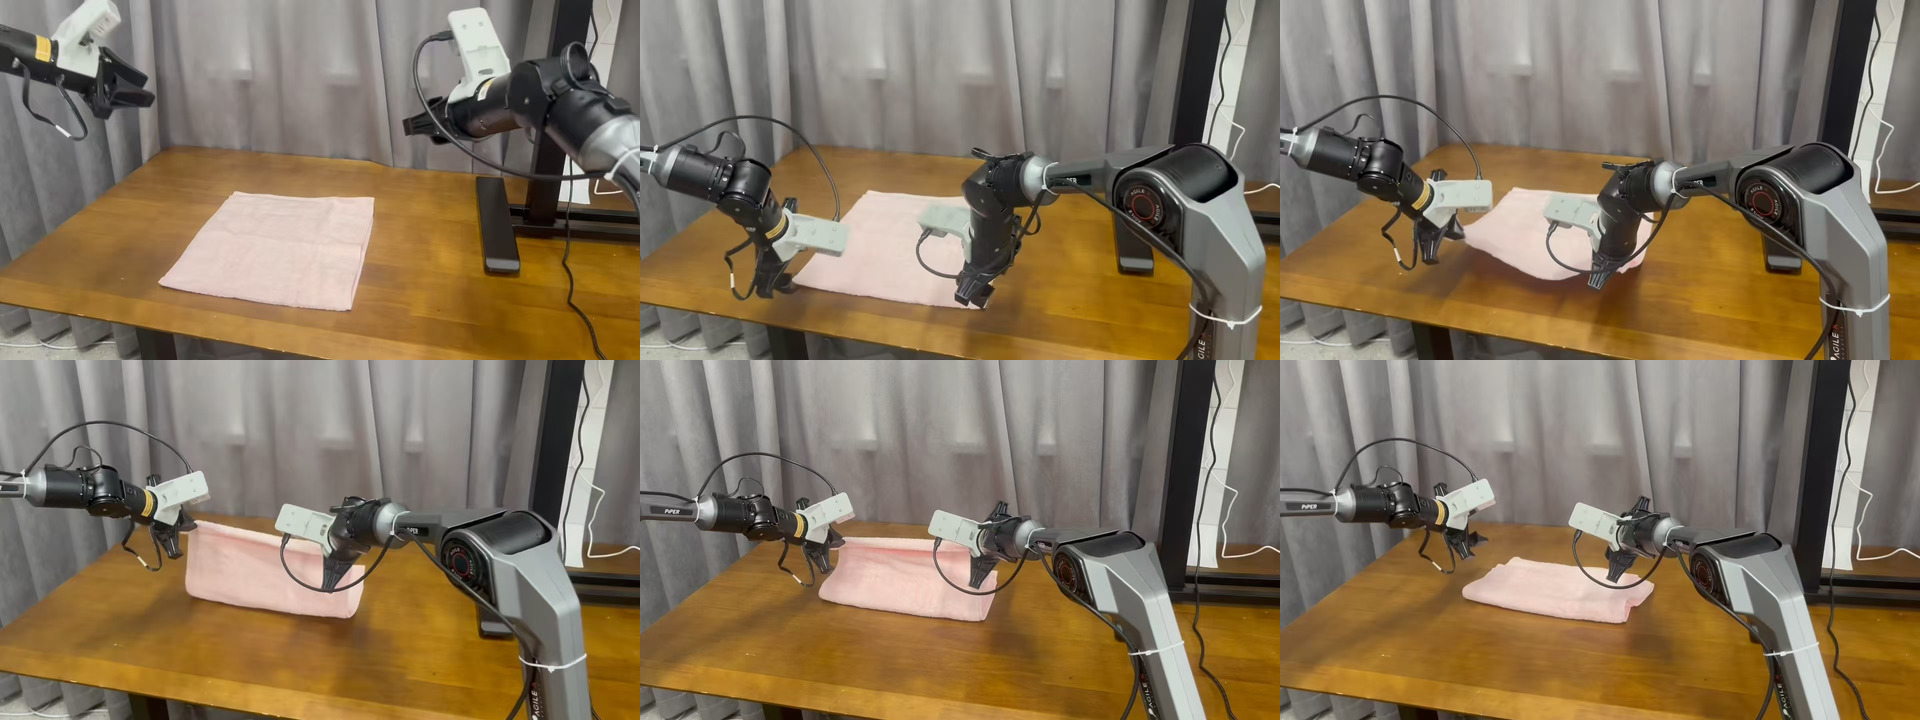
\includegraphics[width=.95\linewidth]{figures/piper_trajectories/towel_contact_sheet.jpg}\par\nointerlineskip
\caption{Piper Semantic task execution. Task instruction: ``Fold the towel from bottom to top.''}
\label{fig:piper-semantic-trajectory}
\par\vspace{\baselineskip}\nointerlineskip
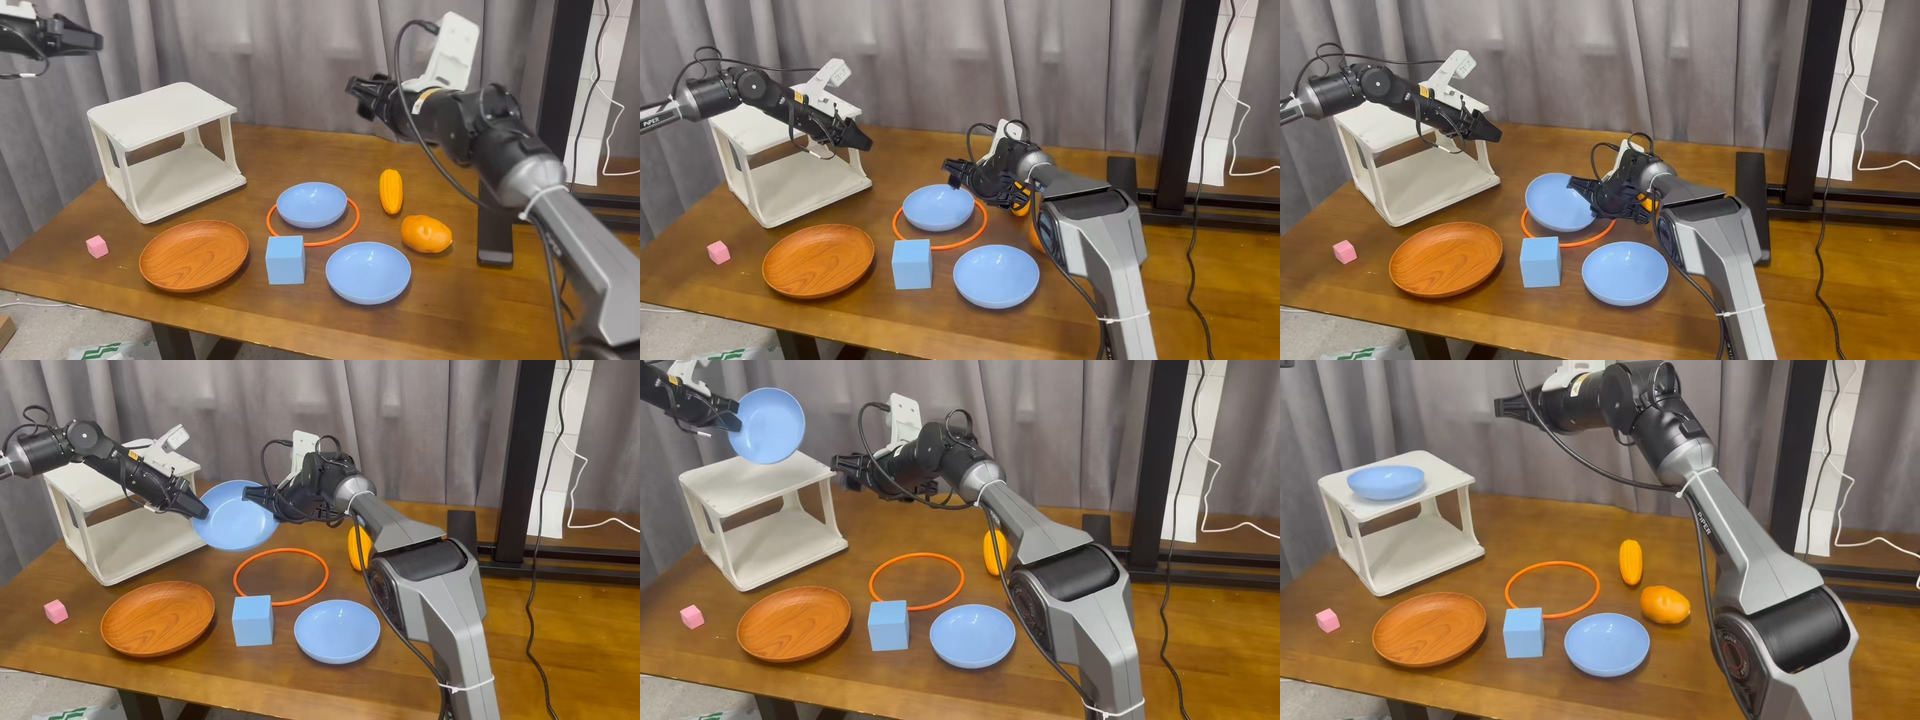
\includegraphics[width=.95\linewidth]{figures/piper_trajectories/spatial_contact_sheet.jpg}\par\nointerlineskip
\caption{Piper Visual Prompt task execution. Task instruction: ``Place the bowl marked by the red circle on the shelf.''}
\label{fig:piper-vis-trajectory}
\par\vspace{\baselineskip}\nointerlineskip
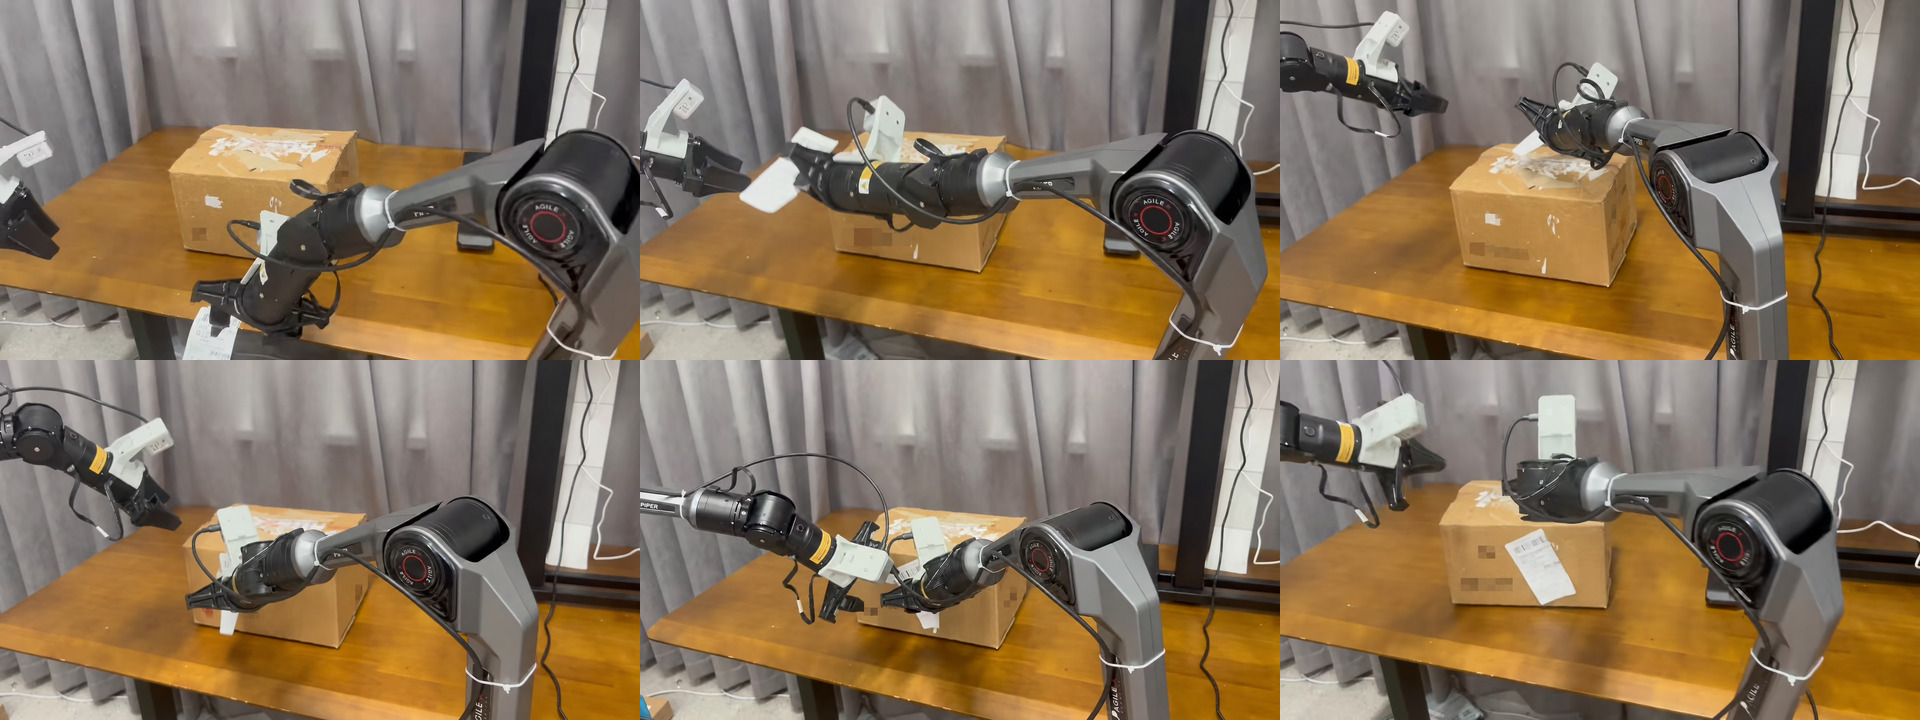
\includegraphics[width=.95\linewidth]{figures/piper_trajectories/control_contact_sheet.jpg}\par\nointerlineskip
\caption{Piper Control task execution. The initial instruction, ``Attach the sticker to the top of the box,'' is replaced during execution by ``Attach the sticker to the front of the box.''}
\label{fig:piper-control-trajectory}
\end{figure}

\clearpage
\hypertarget{limitations-and-future-work}{%
\section{Limitations and Future Work}\label{limitations-and-future-work}}

This work focuses on enabling existing manipulation skills to be
flexibly invoked through diverse instructions, with evaluation covering
representative scenarios involving fine-grained semantic following,
multimodal instruction understanding, and mid-execution corrective control. More open-ended task
spaces, longer-horizon instruction composition, and capability transfer
across robot platforms remain directions for further exploration.
Future work will broaden the coverage of instructions and interaction
scenarios, investigate how instruction-conditioned policies can work
with high-level planning and safe execution mechanisms, and continue to
develop LIBERO-SMART to support broader research on instruction
following and interactive control.

% It remains a working draft: figures, references, final results, and page compression are pending.
\end{document}
